\documentclass[conference]{IEEEtran}
\IEEEoverridecommandlockouts
\usepackage{cite}
\usepackage{amsmath,amssymb,amsfonts}
\usepackage{bm}
\usepackage{algorithmic}
\usepackage{graphicx}
\usepackage{textcomp}
\usepackage{xcolor}
\usepackage{booktabs}
\usepackage{multirow}
\usepackage{array}
\usepackage{tabularx}
\usepackage{makecell}
\usepackage{adjustbox}
\usepackage{url}
\usepackage{hyperref}
\usepackage{balance}

\newcolumntype{Y}{>{\centering\arraybackslash}X}
\newcolumntype{L}{>{\raggedright\arraybackslash}X}

\hypersetup{
  colorlinks=true,
  linkcolor=black,
  citecolor=black,
  urlcolor=black
}

\graphicspath{{paper_assets/figures/}}

\def\BibTeX{{\rm B\kern-.05em{\sc i\kern-.025em b}\kern-.08em
    T\kern-.1667em\lower.7ex\hbox{E}\kern-.125emX}}

\begin{document}

\title{Beyond Controlled-Domain Accuracy: Leakage-Aware Crop Disease
Classification with Calibration and Multilingual Decision Support}

\makeatletter
\newcommand{\linebreakand}{%
  \end{@IEEEauthorhalign}
  \hfill\mbox{}\par
  \mbox{}\hfill\begin{@IEEEauthorhalign}
}
\makeatother

\author{
\IEEEauthorblockN{Prajwal Aaryan Immadi}
\IEEEauthorblockA{\textit{School of Computer Science and Engineering} \\
\textit{VIT-AP University}\\
Amaravati, India \\
prajwal.23bce8631@vitapstudent.ac.in}
\and
\IEEEauthorblockN{Teja Sai Maddirala}
\IEEEauthorblockA{\textit{School of Computer Science and Engineering} \\
\textit{VIT-AP University}\\
Amaravati, India \\
teja.23bce7573@vitapstudent.ac.in}
\linebreakand
\IEEEauthorblockN{Sai Nihar Kunala}
\IEEEauthorblockA{\textit{School of Computer Science and Engineering} \\
\textit{VIT-AP University}\\
Amaravati, India \\
nihar.23bce7213@vitapstudent.ac.in}
%
\and
%
\IEEEauthorblockN{Tanishq S}
\IEEEauthorblockA{\textit{School of Computer Science and Engineering} \\
\textit{VIT-AP University}\\
Amaravati, India \\
tanishq.23bce20211@vitapstudent.ac.in}
\linebreakand
\IEEEauthorblockN{Koduru Hajarathaiah\textsuperscript{*}}
\IEEEauthorblockA{\textit{School of Computer Science and Engineering} \\
\textit{VIT-AP University}\\
Amaravati, India \\
hajarathaiah.k@vitap.ac.in}
}

\IEEEoverridecommandlockouts
\IEEEpubid{\makebox[\columnwidth]{979-8-3315-7436-9/25/\$31.00 ©2025 IEEE
\hfill} \hspace{\columnsep}\makebox[\columnwidth]{ }}

\maketitle
\IEEEpubidadjcol

% Put mentor note at bottom of page 1 (not inside introduction)
\begingroup
\renewcommand\thefootnote{}\footnotetext{\textsuperscript{*}Mentored the research work.}
\endgroup

% =====================================================================
% ABSTRACT
% =====================================================================
\begin{abstract}
Crop disease classification systems trained on controlled laboratory
datasets frequently report near-perfect accuracy yet falter when
exposed to field-acquired imagery. This paper presents a reproducible,
leakage-aware pipeline for 19-class crop disease recognition derived
from a curated PlantVillage subset spanning four crops (bell~pepper,
corn, potato, tomato). The pipeline combines near-duplicate auditing,
frozen three-way data partitioning, convolutional and transformer
classifiers, post-hoc temperature-scaling calibration, confidence-based
selective prediction, a heuristic visible lesion-area proxy, zero-shot
external evaluation on PlantDoc, and a retrieval-grounded multilingual
advisory prototype.

EfficientNet-B0, pre-specified as the baseline model, achieves
99.53\% top-1 accuracy and 0.9929 macro-F1 on the locked 5{,}322-image
internal test set. Temperature scaling ($T\!=\!1.5695$) reduces expected
calibration error (ECE) from 0.0032 to 0.0023 and Brier score from
0.00704 to 0.00642, while internal-test negative log-likelihood
increases slightly from 0.0155 to 0.0159; calibration improvement is
therefore metric-dependent rather than uniform. An EfficientNetV2-S
proposed model and a ViT-B/16 comparator reach comparable internal
accuracy but offer no material advantage under this evaluation protocol.

Zero-shot evaluation on a 144-image, 15-class semantically mapped
PlantDoc subset reveals sharp domain shift: top-1 accuracy drops to
19.44\% while top-5 accuracy remains 67.36\%, indicating that the
correct class is retrievable within the model's top predictions but
is not reliably top-ranked under field-like conditions. Strong
controlled-domain performance did not transfer reliably to the
semantically mapped PlantDoc external subset, demonstrating that high
internal accuracy alone is insufficient evidence of robustness to
field-like imaging conditions.
\end{abstract}

\begin{IEEEkeywords}
crop disease detection, EfficientNet, Vision Transformer, temperature
scaling, calibration, selective prediction, domain shift, PlantDoc,
retrieval-augmented generation, multilingual advisory, PlantVillage
\end{IEEEkeywords}

% =====================================================================
\section{Introduction}
\label{sec:introduction}
% =====================================================================

Crop diseases are responsible for substantial yield losses worldwide,
with estimates from the Food and Agriculture Organization of the
United Nations (FAO) suggesting that plant pathogens and pests account
for up to 40\% of annual global crop production
losses~\cite{savary2019global}. For smallholder farmers
with limited access to extension services, early and accurate disease
identification is a critical determinant of treatment timing and
economic outcome~\cite{ramcharan2017deep}. Automated
computer-vision systems trained on large annotated datasets offer the
potential to democratise field-level disease
diagnosis~\cite{mohanty2016deep,ferentinos2018deep}, particularly
when deployed on mobile platforms accessible in low-connectivity
regions~\cite{ramcharan2017deep,atila2021plant}.

The PlantVillage dataset~\cite{hughes2015open}, comprising over
54{,}000 images collected under controlled, single-leaf conditions
against uniform backgrounds, has become the dominant benchmark for crop
disease classification. Models trained on PlantVillage routinely
achieve accuracies exceeding
95\%~\cite{mohanty2016deep,too2019comparative,kamilaris2018deep}.
However, a growing body of evidence cautions against interpreting such
figures as deployment readiness. Controlled-domain datasets exhibit a
fundamental mismatch with the complex backgrounds, variable lighting,
overlapping leaves, and partial occlusions encountered in real
agricultural
fields~\cite{ferentinos2018deep,barbedo2018factors}.
This domain shift problem has been demonstrated empirically through the
PlantDoc dataset~\cite{singh2020plantdoc}, which provides
field-acquired images and enables direct measurement of the gap between
controlled and field-like performance.

Beyond raw accuracy, well-calibrated confidence estimates are essential
for safe model deployment. Overconfident predictions---wherein the
model assigns high softmax probabilities to incorrect classes---are
particularly hazardous in high-stakes agricultural
decisions~\cite{guo2017calibration}. Temperature
scaling~\cite{guo2017calibration} is a widely used post-hoc
calibration method that rescales logits by a learned scalar, improving
confidence alignment without altering top-1 predictions. Selective
prediction
frameworks~\cite{geifman2017selective} complement
calibration by allowing the model to abstain on low-confidence inputs,
providing a mechanism for reducing error rates at the cost of partial
coverage.

Finally, even when a reliable visual classifier is available, farmers
require actionable guidance in their native
language. Retrieval-augmented generation
(RAG) systems~\cite{lewis2020retrieval} can serve as a structured
advisory interface that grounds responses in vetted agronomic knowledge
bases while enforcing safety constraints against prescriptive pesticide
recommendations.

\subsection{Research Objectives}

This study addresses the following objectives:
\begin{enumerate}
    \item Construct a reproducible, leakage-reduced 19-class crop
          disease classification pipeline on PlantVillage-derived data
          using strict partition isolation.
    \item Evaluate and compare EfficientNet-B0, EfficientNetV2-S, and
          ViT-B/16 classifiers on controlled-domain internal metrics
          and selective prediction behaviour.
    \item Quantify zero-shot domain shift by evaluating the
          pre-specified baseline model on the external PlantDoc test
          set under a transparent semantic mapping protocol.
    \item Introduce a heuristic visible lesion-area proxy with
          explicitly stated limitations as a qualitative
          image-characterisation tool.
    \item Design and functionally test a safety-bounded multilingual
          retrieval-grounded advisory prototype that conditions guidance
          on classifier confidence bands.
\end{enumerate}

\subsection{Contributions}

The principal contributions are:
\begin{itemize}
    \item A reproducible, near-duplicate-audited 19-class data split
          protocol with documented seed, class mapping, and partition
          counts, including transparent reporting of reviewed and
          unreviewed near-duplicate candidates.
    \item Multi-architecture benchmarking on the same frozen
          partitions, showing that under the evaluated models and
          split protocol, larger architectures did not show a
          practically meaningful internal-domain advantage over the
          compact EfficientNet-B0 baseline.
    \item A transparent zero-shot PlantDoc evaluation of the proposed
          pipeline, quantifying the controlled-to-field performance
          gap.
    \item A qualitative heuristic visible lesion-area proxy with
          documented protocol limitations, explicitly precluding
          agronomic or clinical severity claims.
    \item A prototype multilingual retrieval-grounded advisory layer
          functionally tested across all 19 labels in English, Hindi,
          and Telugu, with a tiered confidence-safety policy.
\end{itemize}

% =====================================================================
\section{Related Work}
\label{sec:related}
% =====================================================================

\subsection{Plant Disease Datasets and Benchmarking}

Hughes and Salath\'{e}~\cite{hughes2015open} introduced PlantVillage
as the first large-scale open-access leaf-disease image repository.
Subsequent work has critiqued the controlled capture conditions as
unrepresentative of field
settings~\cite{mohanty2016deep,barbedo2018factors}.
Singh et al.~\cite{singh2020plantdoc} addressed this gap with
PlantDoc, a 2{,}600-image multi-crop dataset collected under natural
field conditions. Additional datasets targeting specific crops,
including
cassava~\cite{mwebaze2019icassava,ramcharan2017deep},
rice, and
tomato~\cite{fuentes2017robust} have been developed, but PlantVillage
remains the standard multi-crop controlled benchmark. Dataset
governance issues such as duplicate images across splits have been
identified as a source of inflated accuracy estimates, motivating
careful
de-duplication~\cite{northcutt2021pervasive,barz2020we}.

\subsection{CNN-Based Plant Disease Classification}

Mohanty et al.~\cite{mohanty2016deep} pioneered the application of
deep CNNs to PlantVillage, achieving 99.35\% accuracy under
colour-augmented training.
Ferentinos~\cite{ferentinos2018deep} reported similarly high accuracy
using AlexNet, VGG, and GoogLeNet variants. The effect of transfer
learning from ImageNet-pretrained weights has been consistently
observed to accelerate convergence and improve final
accuracy~\cite{too2019comparative,kamilaris2018deep}.
Data augmentation strategies including random cropping, horizontal
flipping, brightness jitter, and colour-space transformations are
standard
practice.

\subsection{Efficient Neural Architectures}

Tan and Le introduced EfficientNet~\cite{tan2019efficientnet}, which
applies compound scaling to simultaneously balance network width,
depth, and input resolution. The successor
EfficientNetV2~\cite{tan2021efficientnetv2} further improved training
speed through progressive learning and Fused-MBConv blocks.
Applications in agricultural disease recognition have demonstrated
that EfficientNet variants offer a favourable accuracy-efficiency
tradeoff~\cite{atila2021plant}.

\subsection{Vision Transformers in Agricultural Applications}

Dosovitskiy et al.~\cite{dosovitskiy2021image} introduced the Vision
Transformer (ViT) that processes image patches as token sequences with
self-attention. Data Efficient Image Transformers
(DeiT) addressed ViT's large data
requirement through distillation. ViT and Swin
Transformer have been applied to plant disease
recognition, sometimes matching or exceeding CNN performance on
benchmark
datasets. However,
transformer architectures typically require more parameters per model,
limiting their practical advantage in resource-constrained deployments.

\subsection{Probability Calibration and Selective Prediction}

Calibration refers to the agreement between a model's predicted
confidence and its empirical
accuracy~\cite{guo2017calibration}. Temperature scaling divides all
logits by a positive scalar~$T$ optimised to minimise negative
log-likelihood on a held-out calibration
set~\cite{guo2017calibration,platt1999probabilistic}. Dividing all
logits by a positive scalar preserves their ordering and therefore
preserves the top-1 predicted class; it changes the softmax
probability distribution and associated confidence metrics. Selective
classification~\cite{geifman2017selective}
introduces an abstention option: the model declines to classify inputs
below a chosen confidence threshold, trading coverage for improved
accuracy on the retained subset. Overconfidence under distribution
shift has been highlighted as a critical failure mode for
safety-critical
applications~\cite{ovadia2019can}.

\subsection{Domain Adaptation and External Validation}

The domain gap between controlled-laboratory and field-acquired data
is a well-documented challenge in agricultural computer
vision~\cite{barbedo2018factors}. Approaches
include domain
adaptation,
self-supervised pre-training,
and test-time augmentation. However, direct zero-shot
evaluation---applying a source-domain-trained model to target-domain
data without any adaptation---remains the most conservative and honest
estimate of model robustness under distribution
shift. Several studies have demonstrated
large performance drops when PlantVillage models are evaluated on
field
data~\cite{singh2020plantdoc,fuentes2017robust}.

\subsection{Explainability and Lesion Analysis}

Grad-CAM~\cite{selvaraju2017gradcam} and
SHAP provide model-specific and model-agnostic
attribution, respectively. Lesion segmentation methods range from
threshold-based colour
separation to deep semantic
segmentation. Severity estimation---the
quantification of disease extent within a leaf---typically requires
expert-annotated pixel masks for
validation. In the absence of
validated annotations, any automatic severity estimate must be
characterised as a heuristic proxy.

\subsection{Retrieval-Augmented Advisory Systems}

RAG systems~\cite{lewis2020retrieval} combine a
retrieval module over a curated knowledge base with a language model to
generate grounded responses. Responsible deployment of AI advisory
systems in agriculture requires explicit safety constraints,
uncertainty communication, and avoidance of unverified pesticide or
chemical
recommendations.
Multilingual capability is particularly important for serving
smallholder farmers in South
Asia.

% =====================================================================
\section{Materials and Methods}
\label{sec:methods}
% =====================================================================

\subsection{Datasets, Class Definition, and Data Governance}

The primary dataset is a curated subset of
PlantVillage~\cite{hughes2015open}, selecting five economically
important crop species: bell~pepper (\textit{Capsicum annuum}), corn
(\textit{Zea~mays}), potato (\textit{Solanum tuberosum}), soybean
(\textit{Glycine~max}), and tomato (\textit{Solanum lycopersicum}).
The initial selected-source pool contained \textbf{31{,}729} images
across 20 crop--disease label combinations. Five images identified as
exact validation-set duplicates were removed during exploratory data
analysis, leaving 31{,}724 clean images across 20 classes and 5
crops~(Table~\ref{tab:dataflow}).

The primary classification task, designated \textbf{Main19}, excludes
the \texttt{soybean\_\_healthy} class, which was reserved for a
secondary auxiliary experiment (Aux20). After excluding
\texttt{soybean\_\_healthy} and removing two confirmed near-duplicate
cross-split images (see Section~\ref{sec:duplicate}), the final
Main19 task contains \textbf{19~classes} spanning \textbf{four~crops}:
bell~pepper, corn, potato, and tomato. The 19~labels comprise
4~healthy-state classes and 15~diseased-state classes. The largest
class (tomato yellow leaf curl virus) contains 5{,}357~images; the
smallest (potato healthy) contains 152~images, yielding a class
imbalance ratio of 35.24.

\begin{table}[!t]
\caption{Main19 Dataset Flow. Each row removes a specific set of
images. The final Main19 total is the sum of the three locked
partitions.}
\label{tab:dataflow}
\centering
\small
\begin{tabular}{lr}
\toprule
\textbf{Stage} & \textbf{Images} \\
\midrule
Initial selected-source pool (5~crops, 20~classes) & 31{,}729 \\
$-$ Exact validation-set duplicates & $-5$ \\
$=$ EDA-clean pool & 31{,}724 \\
$-$ Confirmed near-duplicate cross-split exclusions & $-2$ \\
$=$ Final locked pool (Aux20, 20~classes) & 31{,}722 \\
$-$ Excluded class: \texttt{soybean\_\_healthy} & $-5{,}090$ \\
$=$ \textbf{Final Main19 total (19~classes, 4~crops)} & \textbf{26{,}632} \\
\midrule
\quad Training split & 18{,}113 \\
\quad Calibration split & 3{,}197 \\
\quad Locked internal test split & 5{,}322 \\
\bottomrule
\end{tabular}
\end{table}

The external evaluation dataset is
PlantDoc~\cite{singh2020plantdoc}, a field-acquired, multi-crop
leaf-disease dataset. Only the PlantDoc test split was used; no
PlantDoc image was accessed for training, model selection, temperature
fitting, or threshold calibration, ensuring that the PlantDoc
evaluation is strictly zero-shot.

\subsection{Duplicate Auditing and Reproducible Data Splits}
\label{sec:duplicate}

Near-duplicate detection was conducted using perceptual hashing
(pHash) with a Hamming-distance threshold of $\leq 4$~bits, yielding
\textbf{136} near-duplicate candidate
pairs~\cite{zauner2010implementation}. Of these, \textbf{2} were
confirmed as true cross-split near-duplicates and excluded from
all downstream partitions. The remaining \textbf{134} candidate pairs
were flagged for review but remain \textbf{unreviewed} in the
repository audit log. All 136 candidates are cross-split pairs (one
image from the original training pool and one from the original
validation set).

Because the review was not exhaustive, we do not claim that the final
split is completely free of near-duplicate leakage. Rather, the audit
reduced documented leakage risk by identifying and removing the two
highest-similarity confirmed duplicates. The 134 unreviewed candidates
represent a residual risk that could be addressed by future manual or
automated review.

Reproducible three-way stratified splits were constructed at random
seed~7. The original PlantVillage training pool served as the
development pool from which 15\% were stratified-sampled to form the
calibration split. The original PlantVillage validation set was
retained unchanged as the locked internal test set (after the two
near-duplicate exclusions). Partition membership was frozen and saved
as versioned manifests before any model training commenced.

The final locked Main19 partition counts are:
\textbf{training}: 18{,}113 images;
\textbf{calibration}: 3{,}197 images;
\textbf{internal test}: 5{,}322 images.
Fig.~\ref{fig:split_distribution} shows the per-class image counts
across all three partitions.

\begin{figure*}[!t]
    \centering
    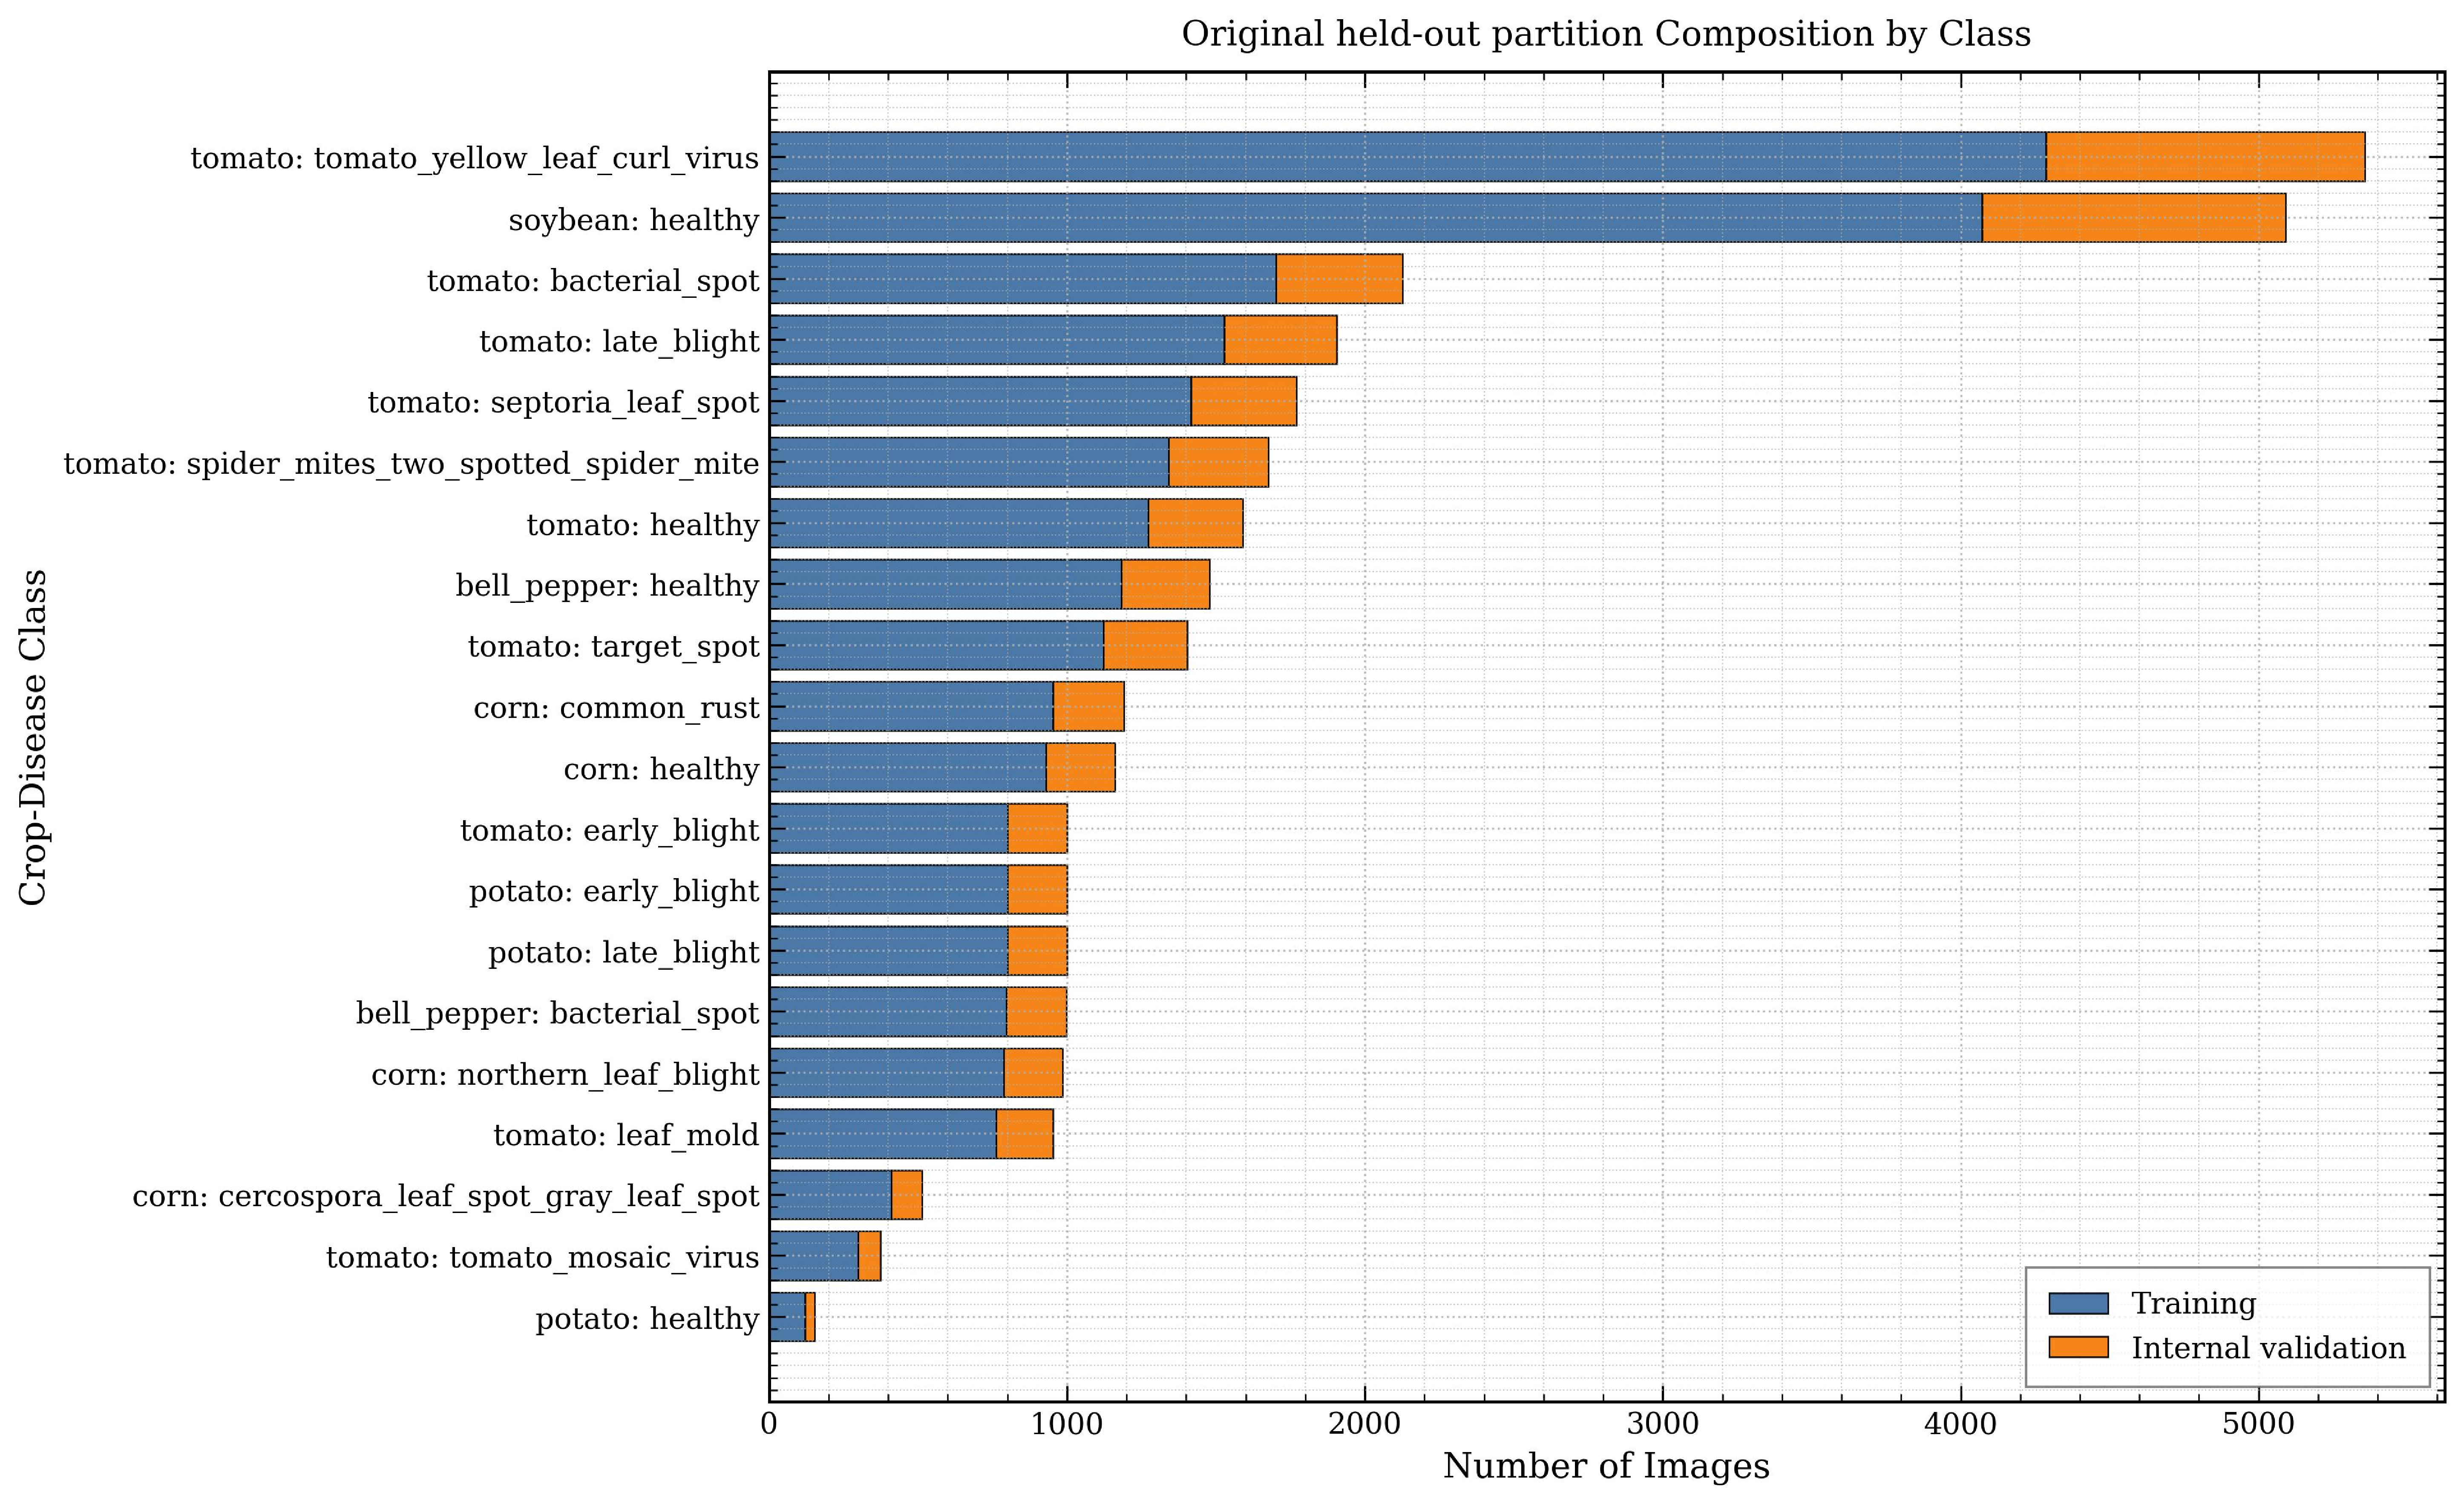
\includegraphics[
        width=0.94\textwidth,
        height=0.42\textheight,
        keepaspectratio
    ]{fig_02_split_distribution.pdf}
    \caption{Image counts per Main19 class across the three frozen
    partitions (training: 18{,}113; calibration: 3{,}197; internal
    test: 5{,}322). Classes are ordered by total size. All partitions
    were stratified by class and their membership frozen before any
    model training. The 19~classes span four crops: bell~pepper~(2),
    corn~(4), potato~(3), and tomato~(10).}
    \label{fig:split_distribution}
\end{figure*}

\subsection{Image Classification Models and Training Protocol}

Three architectures were evaluated on the Main19 task. All models were
initialised with ImageNet-pretrained weights (IMAGENET1K\_V1) and
fine-tuned on the training split. Checkpoint selection for each model
was governed exclusively by calibration-set macro-F1; the internal
test set was not accessed during training or checkpoint selection for
any of the three models. The internal test set was accessed only once,
for final one-shot evaluation after all checkpoints had been frozen.

\textbf{EfficientNet-B0 (Baseline).}
The baseline classifier, pre-specified as the primary model for
downstream calibration, external evaluation, and advisory integration,
uses EfficientNet-B0~\cite{tan2019efficientnet} with a 19-class
linear head. Images were resized to $224\times224$~pixels. Training
used class-weighted cross-entropy loss with
AdamW~\cite{loshchilov2017decoupled} at learning rate
$3\!\times\!10^{-4}$, weight decay $10^{-4}$, batch size~32, and a
maximum of 15~epochs with early stopping after 4~non-improving
calibration epochs. Step-decay halved the learning rate at epochs~6
and~13. The final checkpoint was selected at epoch~15 (calibration
macro-F1: 0.9940). Notebook metadata confirms
\texttt{internal\_test\_used:~false}.

\textbf{EfficientNetV2-S (Proposed).}
The proposed model replaces the backbone with
EfficientNetV2-S~\cite{tan2021efficientnetv2}. Input resolution was
increased to $384\times384$~pixels. Training used class-weighted focal
cross-entropy loss~\cite{lin2017focal} ($\gamma\!=\!1.5$) with AdamW
at learning rate $2\!\times\!10^{-4}$, weight decay $10^{-4}$, batch
size~12, and a maximum of 20~epochs (early stopping patience:~5). The
best checkpoint was selected at epoch~13 (calibration macro-F1:
0.9979). Notebook metadata confirms
\texttt{internal\_test\_used:~false}.

\textbf{ViT-B/16 (Architecture Comparator).}
Vision Transformer ViT-B/16~\cite{dosovitskiy2021image} was trained as
an architecture comparator. Input size was $224\times224$. Training
used class-weighted cross-entropy with label smoothing
($\varepsilon\!=\!0.05$)~\cite{szegedy2016rethinking} and AdamW at
learning rate $10^{-4}$, weight decay $10^{-4}$, batch size~16, and a
maximum of 15~epochs (early stopping patience:~4). The best checkpoint
was selected at epoch~11 (calibration macro-F1: 0.9947). Notebook
metadata confirms
\texttt{internal\_test\_used\_during\_training:~false}.

All experiments were conducted in PyTorch~2.10.0+cu128,
Python~3.12.13, NumPy~2.0.2, and pandas~2.3.3 at seed~7. Training was
performed on NVIDIA GPU hardware via the Kaggle platform.
Table~\ref{tab:architecture} summarises the model configurations.

\begin{table*}[!t]
\caption{Model Architectures and Training Configurations. Wtd.\ CE
denotes class-weighted cross-entropy; LS denotes label smoothing; ES
denotes early stopping. All checkpoints were selected by
calibration-set macro-F1. The internal test set was not used for
checkpoint selection in any model.}
\label{tab:architecture}
\centering
\small
\setlength{\tabcolsep}{5pt}
\renewcommand{\arraystretch}{1.12}
\begin{tabularx}{\textwidth}{L Y Y Y}
\toprule
\textbf{Property} & \textbf{EfficientNet-B0} & \textbf{EfficientNetV2-S} & \textbf{ViT-B/16} \\
\midrule
Input size & $224\times224$ & $384\times384$ & $224\times224$ \\
Parameters & $\approx 5.3$\,M & $\approx 20.2$\,M & 85.8\,M \\
Loss & Wtd.\ CE & Wtd.\ Focal CE & Wtd.\ CE + LS \\
Focal $\gamma$ & --- & 1.5 & --- \\
Label smoothing & None & None & 0.05 \\
Optimiser & AdamW & AdamW & AdamW \\
Learning rate & $3\times10^{-4}$ & $2\times10^{-4}$ & $1\times10^{-4}$ \\
Weight decay & $1\times10^{-4}$ & $1\times10^{-4}$ & $1\times10^{-4}$ \\
Batch size & 32 & 12 & 16 \\
Maximum epochs & 15 & 20 & 15 \\
ES patience & 4 & 5 & 4 \\
Selected epoch & 15 & 13 & 11 \\
Calibration macro-F1 & 0.9940 & 0.9979 & 0.9947 \\
\bottomrule
\end{tabularx}
\end{table*}

\subsection{Post-hoc Calibration}

Following Guo et al.~\cite{guo2017calibration}, temperature scaling
was applied to the EfficientNet-B0 baseline by fitting a scalar
temperature parameter~$T$ that minimises negative log-likelihood on
the calibration split. The optimal temperature was
$T\!=\!1.5695$. Because dividing all logits by a positive scalar
preserves their ordering, the top-1 class assignment is invariant to
temperature scaling: accuracy and macro-F1 are identical before and
after scaling. The transformation changes the softmax probability
distribution and therefore affects confidence-dependent metrics
(ECE, Brier score, NLL).

Expected calibration error (ECE)~\cite{naeini2015obtaining} was
computed with 15~equal-width bins. Brier score~\cite{brier1950verification}
was computed as the mean squared error between predicted probability
vectors and one-hot targets, averaged over samples:
$\text{Brier} = \frac{1}{N}\sum_{i=1}^{N}\sum_{c=1}^{C}(p_{ic} - y_{ic})^2$.

Temperature-scaled internal-test metrics were extracted only for
EfficientNet-B0 (Notebook~04). Independent temperature-scaled
internal-test evaluation for EfficientNetV2-S was not conducted;
accordingly, no temperature-scaled test comparison across models is
reported.

\subsection{Selective Prediction}

Selective prediction was implemented for all three architectures
following the risk--coverage framework of Geifman and
El-Yaniv~\cite{geifman2017selective}. A confidence threshold
$\bm{\tau}$ was selected on the calibration split under the constraint
that the calibration-set error rate (risk) was $\leq 1\%$ while
maximising coverage, with a minimum threshold floor of $\bm{\tau}
\geq 0.50$. Thresholds were selected exclusively on calibration data;
the internal test set was not used for threshold tuning.

For all three models, the selected threshold was
$\bm{\tau}\!=\!0.50$, which is the minimum floor. The confidence
values used for selective prediction are the raw (uncalibrated)
softmax outputs from each model's respective checkpoint; temperature
scaling was not applied before selective prediction thresholding.

\subsection{Heuristic Visible Lesion-Area Proxy}

A heuristic image-based visible lesion-area proxy was computed for all
Main19 images (including healthy classes). The image-processing
procedure estimates the proportion of visible pixels satisfying
pre-defined lesion-like colour and texture criteria, applying
background separation followed by HSV/Lab abnormal-colour and
low-green vegetation heuristics. The method requires no separate
lesion segmentation model and no expert annotation.

The proxy assigns each image to one of three ordinal bands:
\textit{mild\_proxy} ($<5\%$ visible lesion area),
\textit{moderate\_proxy} ($5$--$20\%$), and \textit{severe\_proxy}
($>20\%$). These labels are visual-heuristic designations only. The
protocol metadata explicitly states that the proxy: (i)~is not
expert-annotated lesion segmentation; (ii)~is not a clinical
disease-stage label; (iii)~has not been validated against agronomic
treatment thresholds; and (iv)~does not account for hidden lesions,
leaf age, whole-plant burden, or temporal progression. All proxy
values in this paper are accordingly qualified as heuristic estimates.

This procedure does not identify causal model features and does not
constitute classifier-attention analysis or model-specific
explainability. It is an exploratory image-characterisation measure.

\subsection{Zero-Shot External-Domain Evaluation}
\label{sec:plantdoc_method}

To measure the practical impact of source-to-target domain shift, the
EfficientNet-B0 baseline was applied zero-shot to the PlantDoc test
split. ``Zero-shot'' means no PlantDoc image was used for training,
model selection, calibration, or threshold tuning. EfficientNet-B0 was
pre-specified as the baseline model before internal-test evaluation;
the decision to use it for external evaluation did not depend on
internal-test results.

PlantDoc organises images into 27 folder categories. Of these,
\textbf{15} could be \textit{semantically mapped} to Main19 classes
based on folder names and disease terminology. The remaining 12
folders cover crops absent from Main19 (apple, blueberry, cherry,
grape, peach, raspberry, soybean, squash, strawberry) and were
excluded. Two mappings rely on assumptions about generic folder names:
\texttt{Tomato\_leaf} was mapped to
\texttt{tomato\_\_healthy} and \texttt{Bell\_pepper\_leaf} to
\texttt{bell\_pepper\_\_healthy}. These folder-to-healthy mappings are
semantic assumptions that could affect class-level metrics if the
folders contain non-healthy images.

Evaluation was conducted on the model's unscaled softmax outputs
(temperature $T\!=\!1.0$). Temperature scaling fitted on PlantVillage
calibration data was not applied to PlantDoc, because its application
to a different data distribution is an unjustified extrapolation.

The model outputs predictions across all 19~Main19 classes, but only
15~of those classes have corresponding PlantDoc true labels. The
confusion matrix therefore has 15~true-label rows; predictions into
the remaining 4~Main19 classes (those without PlantDoc counterparts)
are visible in the confusion matrix columns as off-diagonal entries.

\subsection{Retrieval-Grounded Multilingual Advisory Prototype}

The retrieval-grounded advisory prototype provides safety-bounded
educational guidance following a predicted diagnosis. It is not an
image classifier and does not alter classification outputs. The
knowledge base contains 19~entries, one per Main19 label, with
structured agronomic content including symptom descriptions, causal
agents, management principles, and prevention guidelines. All entries
were authored for this project and have not been reviewed or endorsed
by professional plant pathologists.

Retrieval uses TF-IDF cosine similarity with classifier-label
prioritisation~\cite{robertson2009bm25}: when a classifier label is
provided, that entry is retrieved directly. Because there is one entry
per label, correct primary retrieval is deterministic rather than a
competitive search over a large corpus. Responses are generated in
three languages: English, Hindi, and Telugu.

The advisory layer enforces a tiered confidence-safety policy:
\textit{low confidence} ($<0.70$): requests clearer images and expert
confirmation; \textit{medium confidence} ($0.70$--$0.89$): provides
screening-level guidance and recommends inspecting multiple plants;
\textit{high confidence} ($\geq 0.90$): provides substantive
agronomic guidance with mandatory field-verification warnings. Across
all tiers, the system explicitly prohibits pesticide brand, dosage, or
location-specific chemical recommendations.

% =====================================================================
\section{Results}
\label{sec:results}
% =====================================================================

\subsection{Dataset Characteristics and Split Integrity}

The Main19 split yielded 18{,}113 training, 3{,}197 calibration, and
5{,}322 internal test images across 19~classes and 4~crops
(Table~\ref{tab:dataflow}). Stratification preserved the class
proportions across all three partitions
(Fig.~\ref{fig:split_distribution}). Near-duplicate auditing
confirmed 2~cross-split near-duplicate pairs from 136~pHash
candidates. Both were excluded. The remaining 134~candidates are
unreviewed.

\subsection{Controlled-Domain Classification Performance}

\textbf{EfficientNet-B0 Baseline.}
The baseline model achieves \textbf{99.53\%} top-1 accuracy,
99.32\% balanced accuracy, and \textbf{0.9929} macro-F1 on the locked
internal test set (source: Notebook~04 test evaluation).
Fig.~\ref{fig:learning_curves} shows the training and calibration
loss and macro-F1 across 15~epochs. Training converged steadily;
calibration macro-F1 reached 0.9940 at the final epoch, which was
selected as the best checkpoint.

\begin{figure*}[!t]
    \centering
    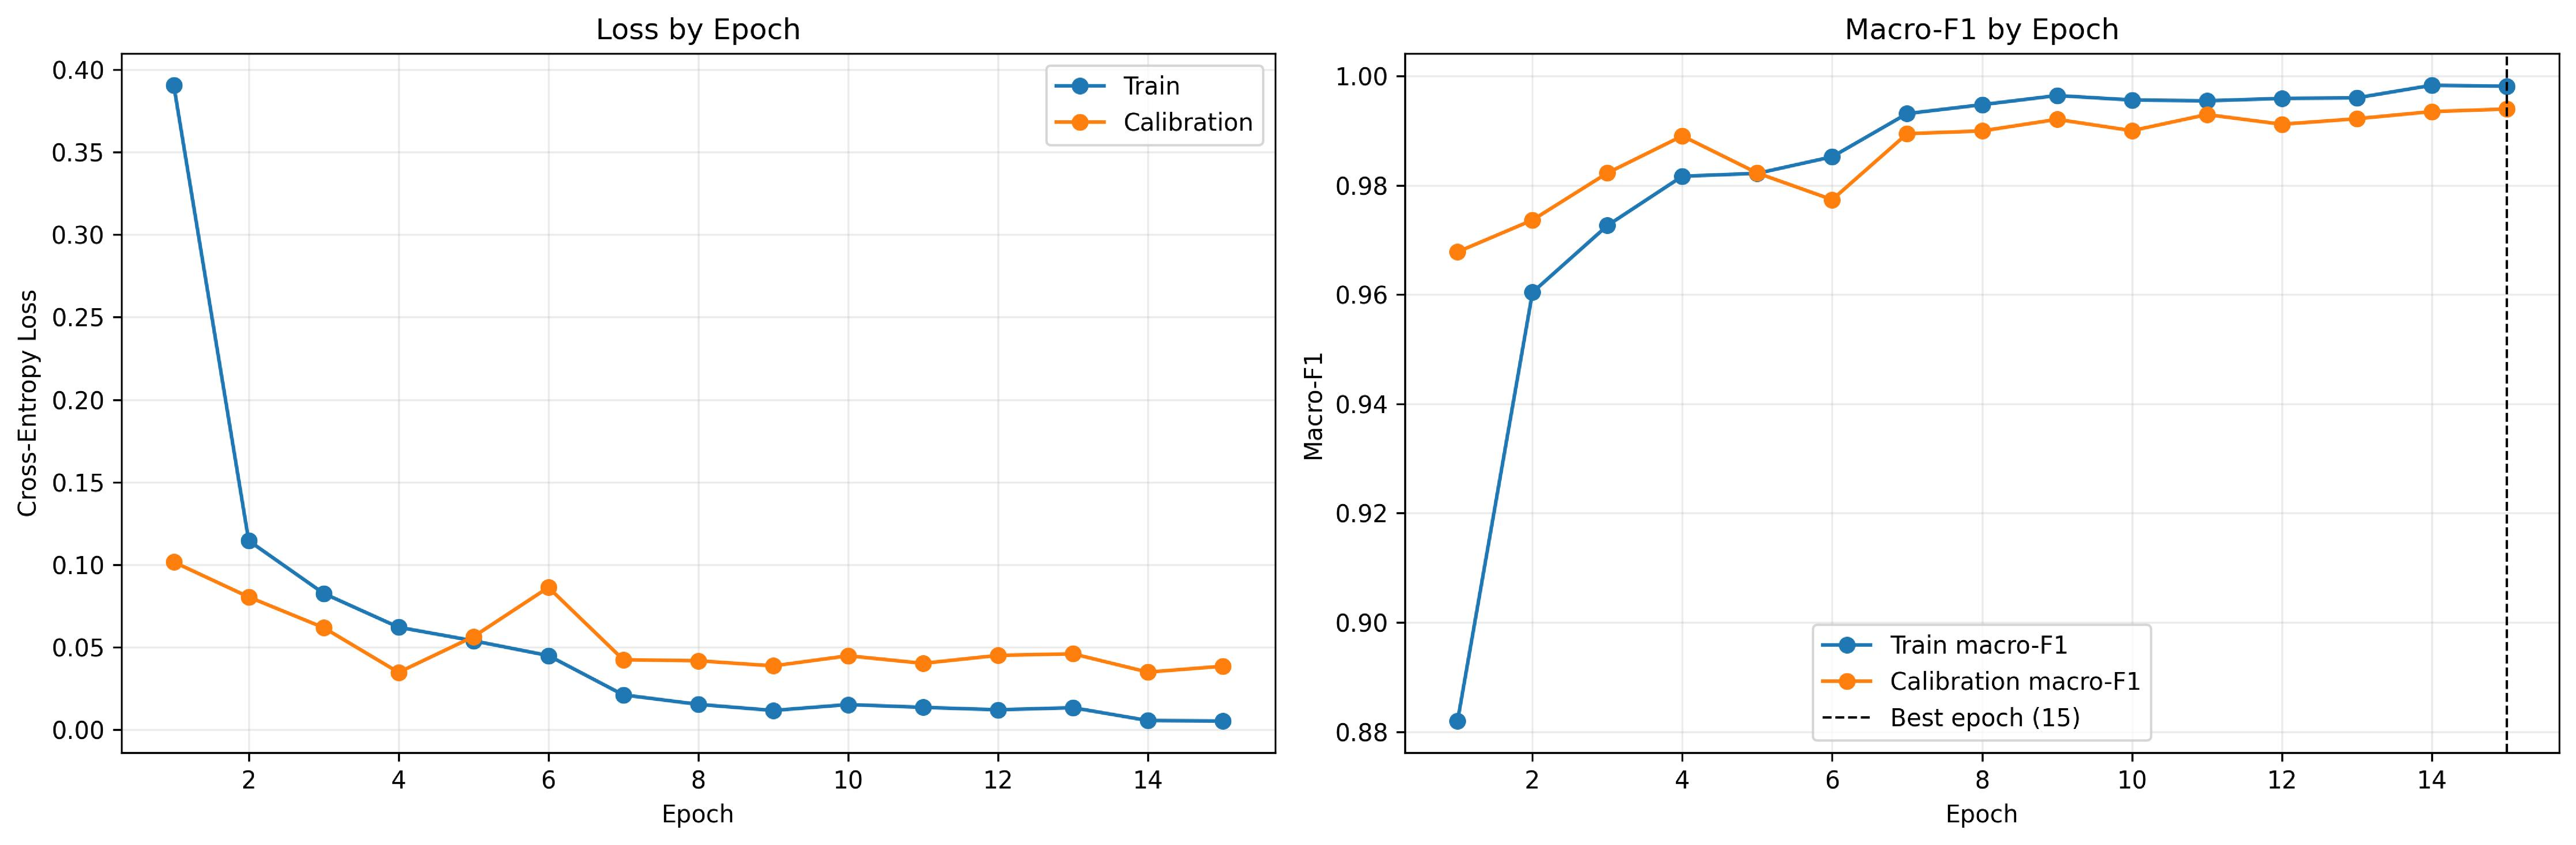
\includegraphics[
        width=0.94\textwidth,
        height=0.40\textheight,
        keepaspectratio
    ]{fig_03_baseline_learning_curves.pdf}
    \caption{EfficientNet-B0 optimisation on the Main19 development
    protocol. Left: training and calibration loss. Right: macro-F1 by
    epoch. The selected checkpoint corresponds to the highest
    calibration macro-F1 (0.9940 at epoch~15). The internal test
    partition was not used for epoch selection (18{,}113~training
    images, 3{,}197~calibration images).}
    \label{fig:learning_curves}
\end{figure*}

\textbf{Multi-Architecture Comparison.}
A post-hoc descriptive comparison was conducted in Notebook~07,
evaluating all three frozen checkpoints on the same locked internal
test set. This comparison was descriptive only; the EfficientNet-B0
baseline had been pre-specified as the primary model before
internal-test evaluation. Table~\ref{tab:internal_comparison}
presents the results.

\begin{table*}[!t]
\caption{Controlled-Domain Performance on the Main19 Internal Test Set
(5{,}322~images). Higher is better for accuracy, balanced accuracy,
and macro-F1; lower is better for NLL. B0 canonical values from the
dedicated evaluation (Notebook~04); V2-S and ViT-B/16 from the
post-hoc comparison (Notebook~07). See text for cross-notebook
discrepancy discussion.}
\label{tab:internal_comparison}
\centering
\small
\setlength{\tabcolsep}{7pt}
\renewcommand{\arraystretch}{1.12}
\begin{tabular}{lccccc}
\toprule
\textbf{Model} & \textbf{Source} & \textbf{Accuracy} & \textbf{Balanced Acc.} & \textbf{Macro-F1} & \textbf{NLL} \\
\midrule
EfficientNet-B0 & NB04 (canonical) & 0.9953 & 0.9932 & 0.9929 & 0.0155 \\
EfficientNet-B0 & NB07 (comparison) & 0.9955 & 0.9935 & 0.9931 & 0.0159 \\
EfficientNetV2-S & NB07 & 0.9955 & 0.9935 & 0.9926 & 0.0176 \\
ViT-B/16 & NB07 & 0.9936 & 0.9938 & 0.9926 & 0.1481 \\
\bottomrule
\end{tabular}
\end{table*}

\textbf{Cross-notebook metric discrepancy.}
The EfficientNet-B0 accuracy differs between Notebook~04 (0.9953025)
and the Notebook~07 comparison table (0.9954904), a difference of one
additional correct prediction out of 5{,}322. The Brier scores also
differ substantially: Notebook~04 reports~0.00704, while Notebook~07
reports~0.000337. This 20-fold discrepancy indicates that the two
notebooks use different Brier score computation implementations. We
adopt the Notebook~04 values as canonical for EfficientNet-B0, because
Notebook~04 is the dedicated temperature-scaling and test-evaluation
notebook and its Brier formula is documented as the standard
multiclass definition. The Brier values from the Notebook~07
comparison table are not directly comparable to Notebook~04 and are
therefore not used for cross-model calibration claims.

Under the evaluated models and split protocol, larger architectures
did not show a practically meaningful internal-domain advantage over
EfficientNet-B0: all three models achieved accuracy above 99.3\% and
macro-F1 above 0.992, while EfficientNet-B0 has approximately
$16\times$ fewer parameters than ViT-B/16.

\subsection{Calibration and Confidence-Aware Prediction}

\textbf{Temperature Scaling.}
Temperature scaling with $T\!=\!1.5695$ preserved accuracy (0.9953)
and macro-F1 (0.9929) identically, reduced internal-test ECE from
0.00321 to 0.00228 (a 29\% relative reduction), and reduced Brier
score from 0.00704 to 0.00642. However, internal-test NLL
\textit{increased slightly} from 0.01550 to 0.01593. Calibration
improvement was therefore metric-dependent rather than uniform.
Table~\ref{tab:calibration_summary} presents the full profile.

\begin{table*}[!t]
\caption{EfficientNet-B0 Calibration Results Before and After
Temperature Scaling ($T\!=\!1.5695$). Accuracy and macro-F1 are
unchanged because positive logit scaling preserves class ranking.
Lower values are better for NLL, Brier score, and ECE. ECE computed
with 15~equal-width bins. Brier: multiclass mean squared error,
$\frac{1}{N}\sum_i\sum_c(p_{ic}-y_{ic})^2$.}
\label{tab:calibration_summary}
\centering
\small
\setlength{\tabcolsep}{9pt}
\renewcommand{\arraystretch}{1.12}
\begin{tabular}{llcccc}
\toprule
\textbf{Split} & \textbf{Scaling} & \textbf{Accuracy} & \textbf{NLL} & \textbf{Brier score} & \textbf{ECE} \\
\midrule
\multirow{2}{*}{Calibration} & Uncalibrated & 0.9959 & 0.01850 & 0.00699 & 0.00392 \\
 & Temperature-scaled & 0.9959 & 0.01830 & 0.00678 & 0.00130 \\
\midrule
\multirow{2}{*}{Internal test} & Uncalibrated & 0.9953 & 0.01550 & 0.00704 & 0.00321 \\
 & Temperature-scaled & 0.9953 & 0.01593 & 0.00642 & \textbf{0.00228} \\
\bottomrule
\end{tabular}
\end{table*}

The reliability diagram (Fig.~\ref{fig:reliability}) confirms that
the temperature-scaled model exhibits closer alignment between mean
confidence bins and empirical accuracy on the internal test set.

\begin{figure}[!t]
    \centering
    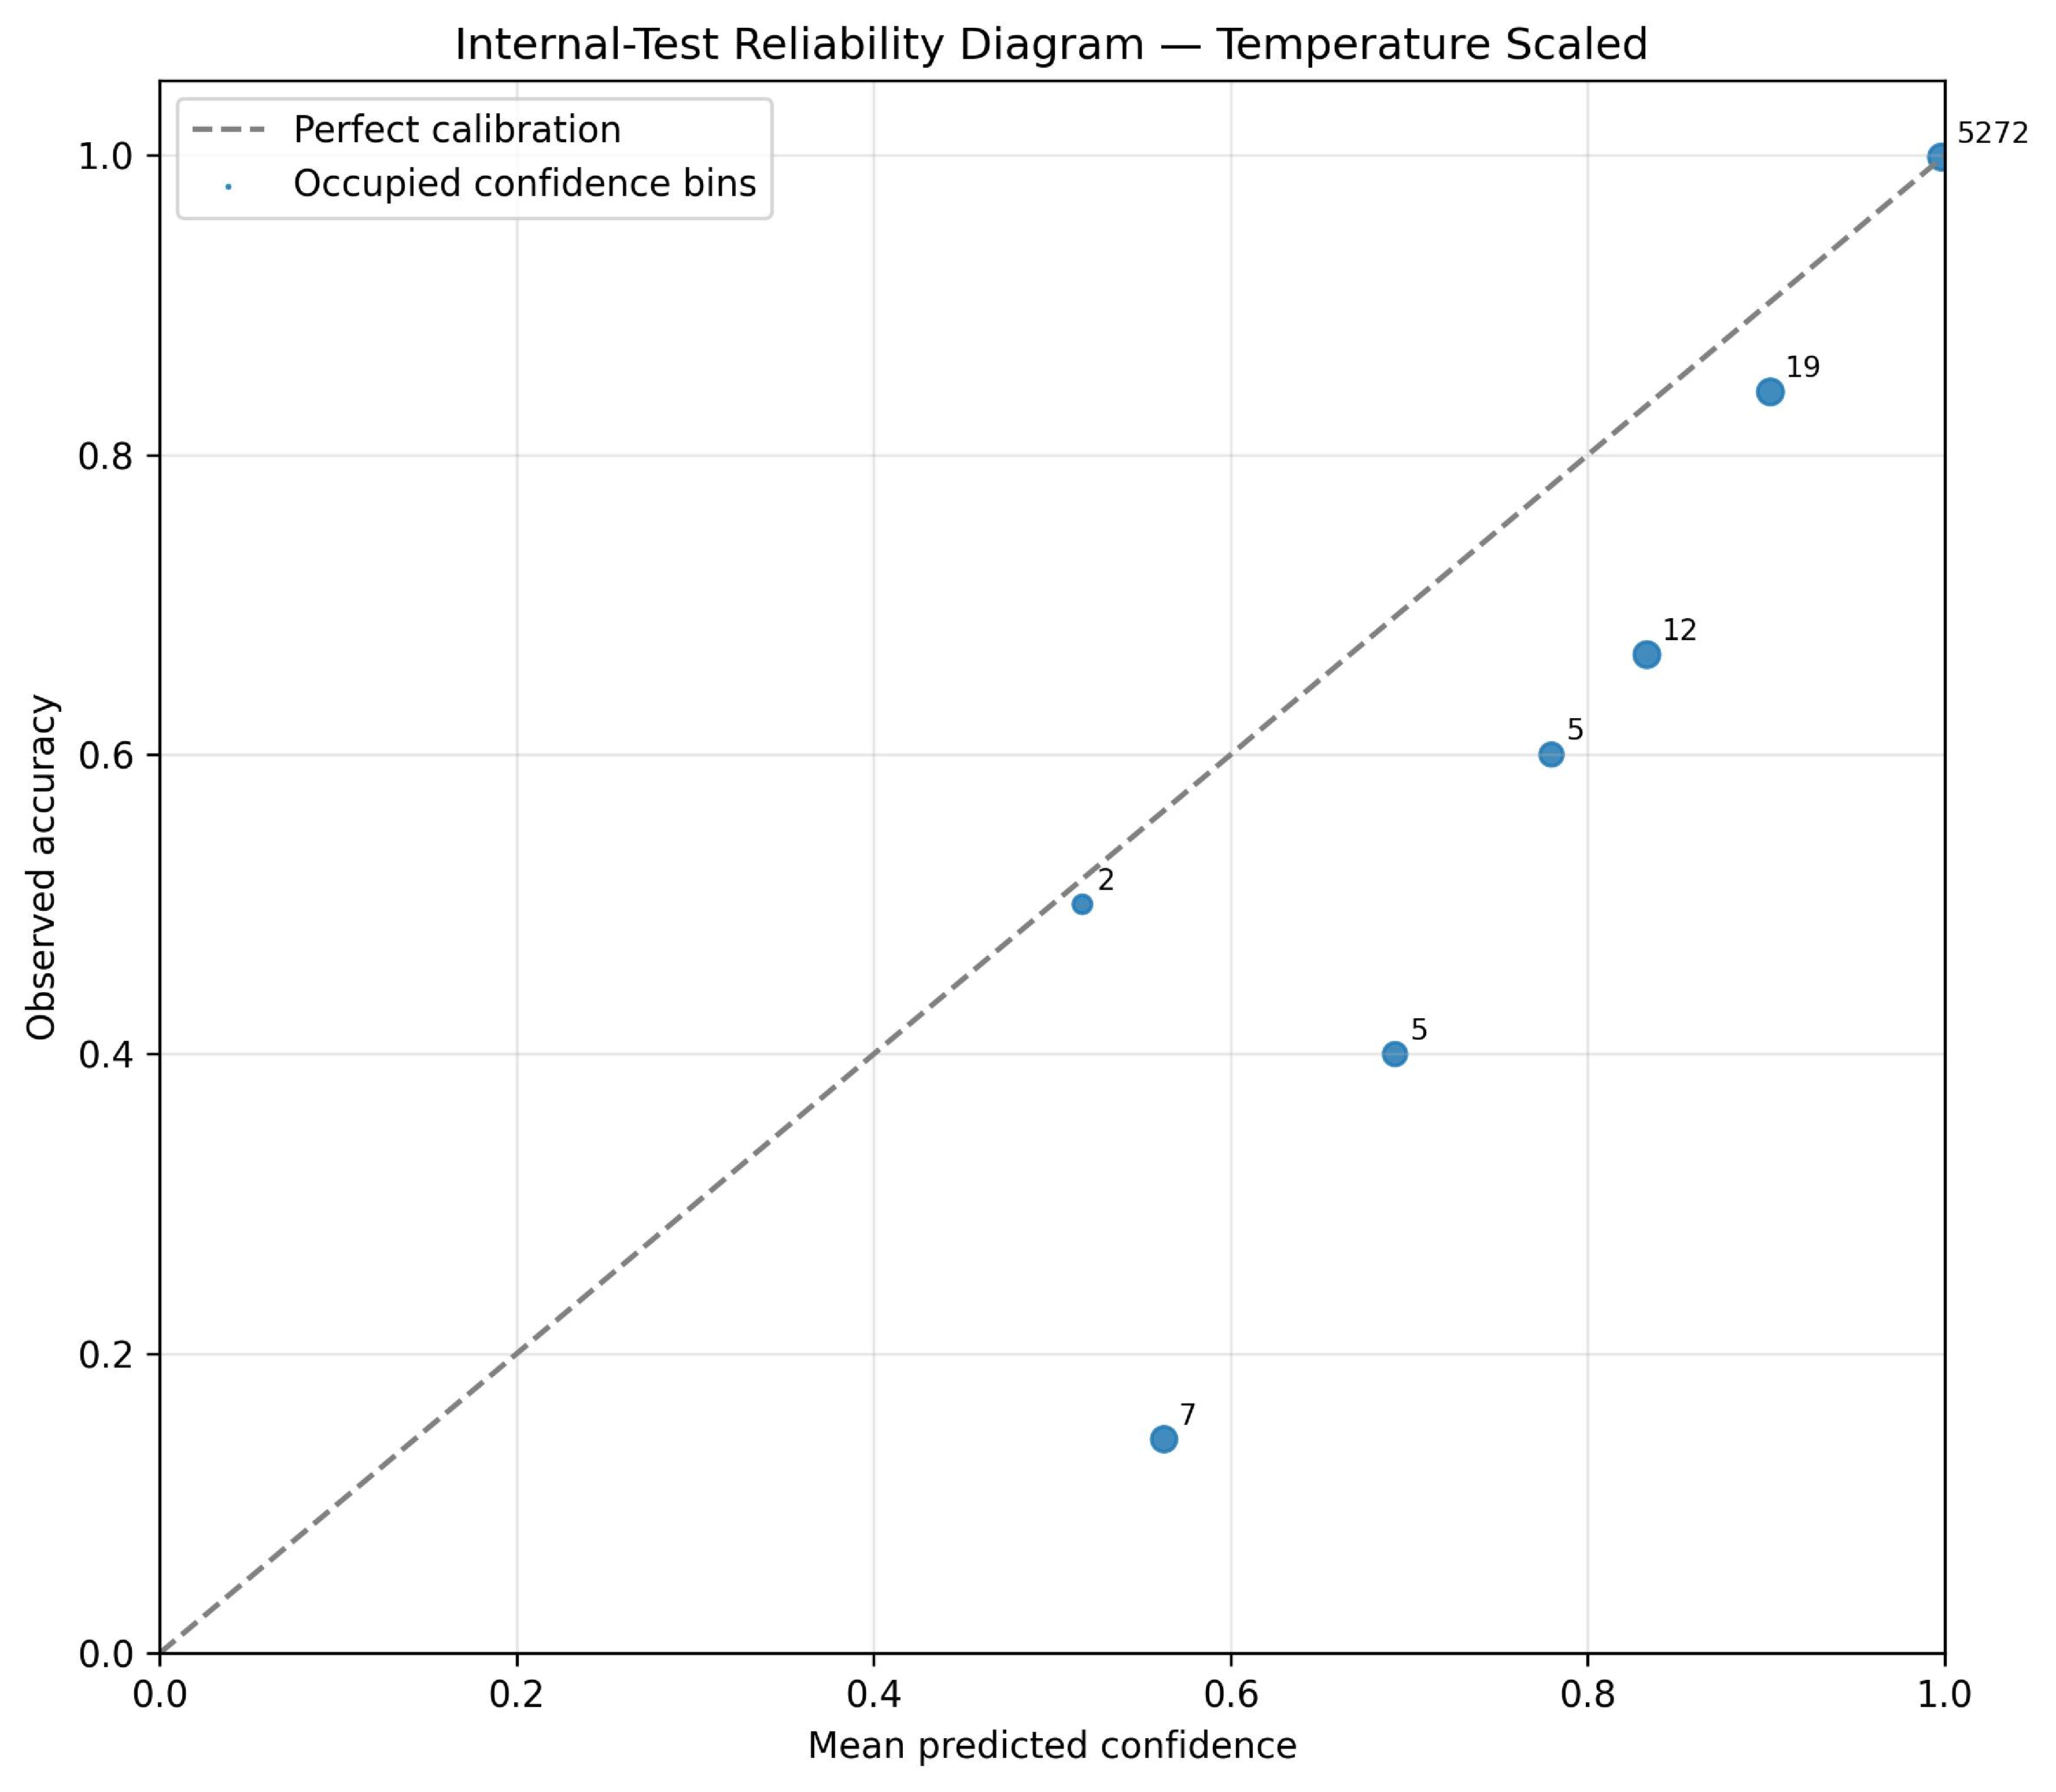
\includegraphics[
        width=\columnwidth,
        height=0.34\textheight,
        keepaspectratio
    ]{fig_04_test_reliability_calibrated.pdf}
    \caption{EfficientNet-B0 reliability diagram on the internal test
    set after temperature scaling ($T\!=\!1.5695$, 15~equal-width
    bins). ECE: 0.0023. The model closely tracks the identity
    diagonal, indicating well-calibrated confidence on the
    source-domain test data.}
    \label{fig:reliability}
\end{figure}

\textbf{Selective Prediction.}
For all three models, the calibration-selected threshold was
$\bm{\tau}\!=\!0.50$ (the minimum floor). At this threshold,
EfficientNet-B0 retained all 5{,}322 internal test images
(coverage:~100\%), achieving selective accuracy of 0.9955 and risk of
0.0045. EfficientNetV2-S rejected 2~images (coverage:~99.96\%),
ViT-B/16 rejected 3 (coverage:~99.94\%). At the
calibration-selected threshold, EfficientNet-B0 retained all
internal-test images because predictions on the matched internal
domain were already highly confident. Accordingly, the reject option
produced no additional in-domain benefit for this model.

Fig.~\ref{fig:risk_coverage} shows the risk--coverage curves on the
internal test set. Table~\ref{tab:selective} summarises the selective
prediction results.

\begin{figure*}[!t]
    \centering
    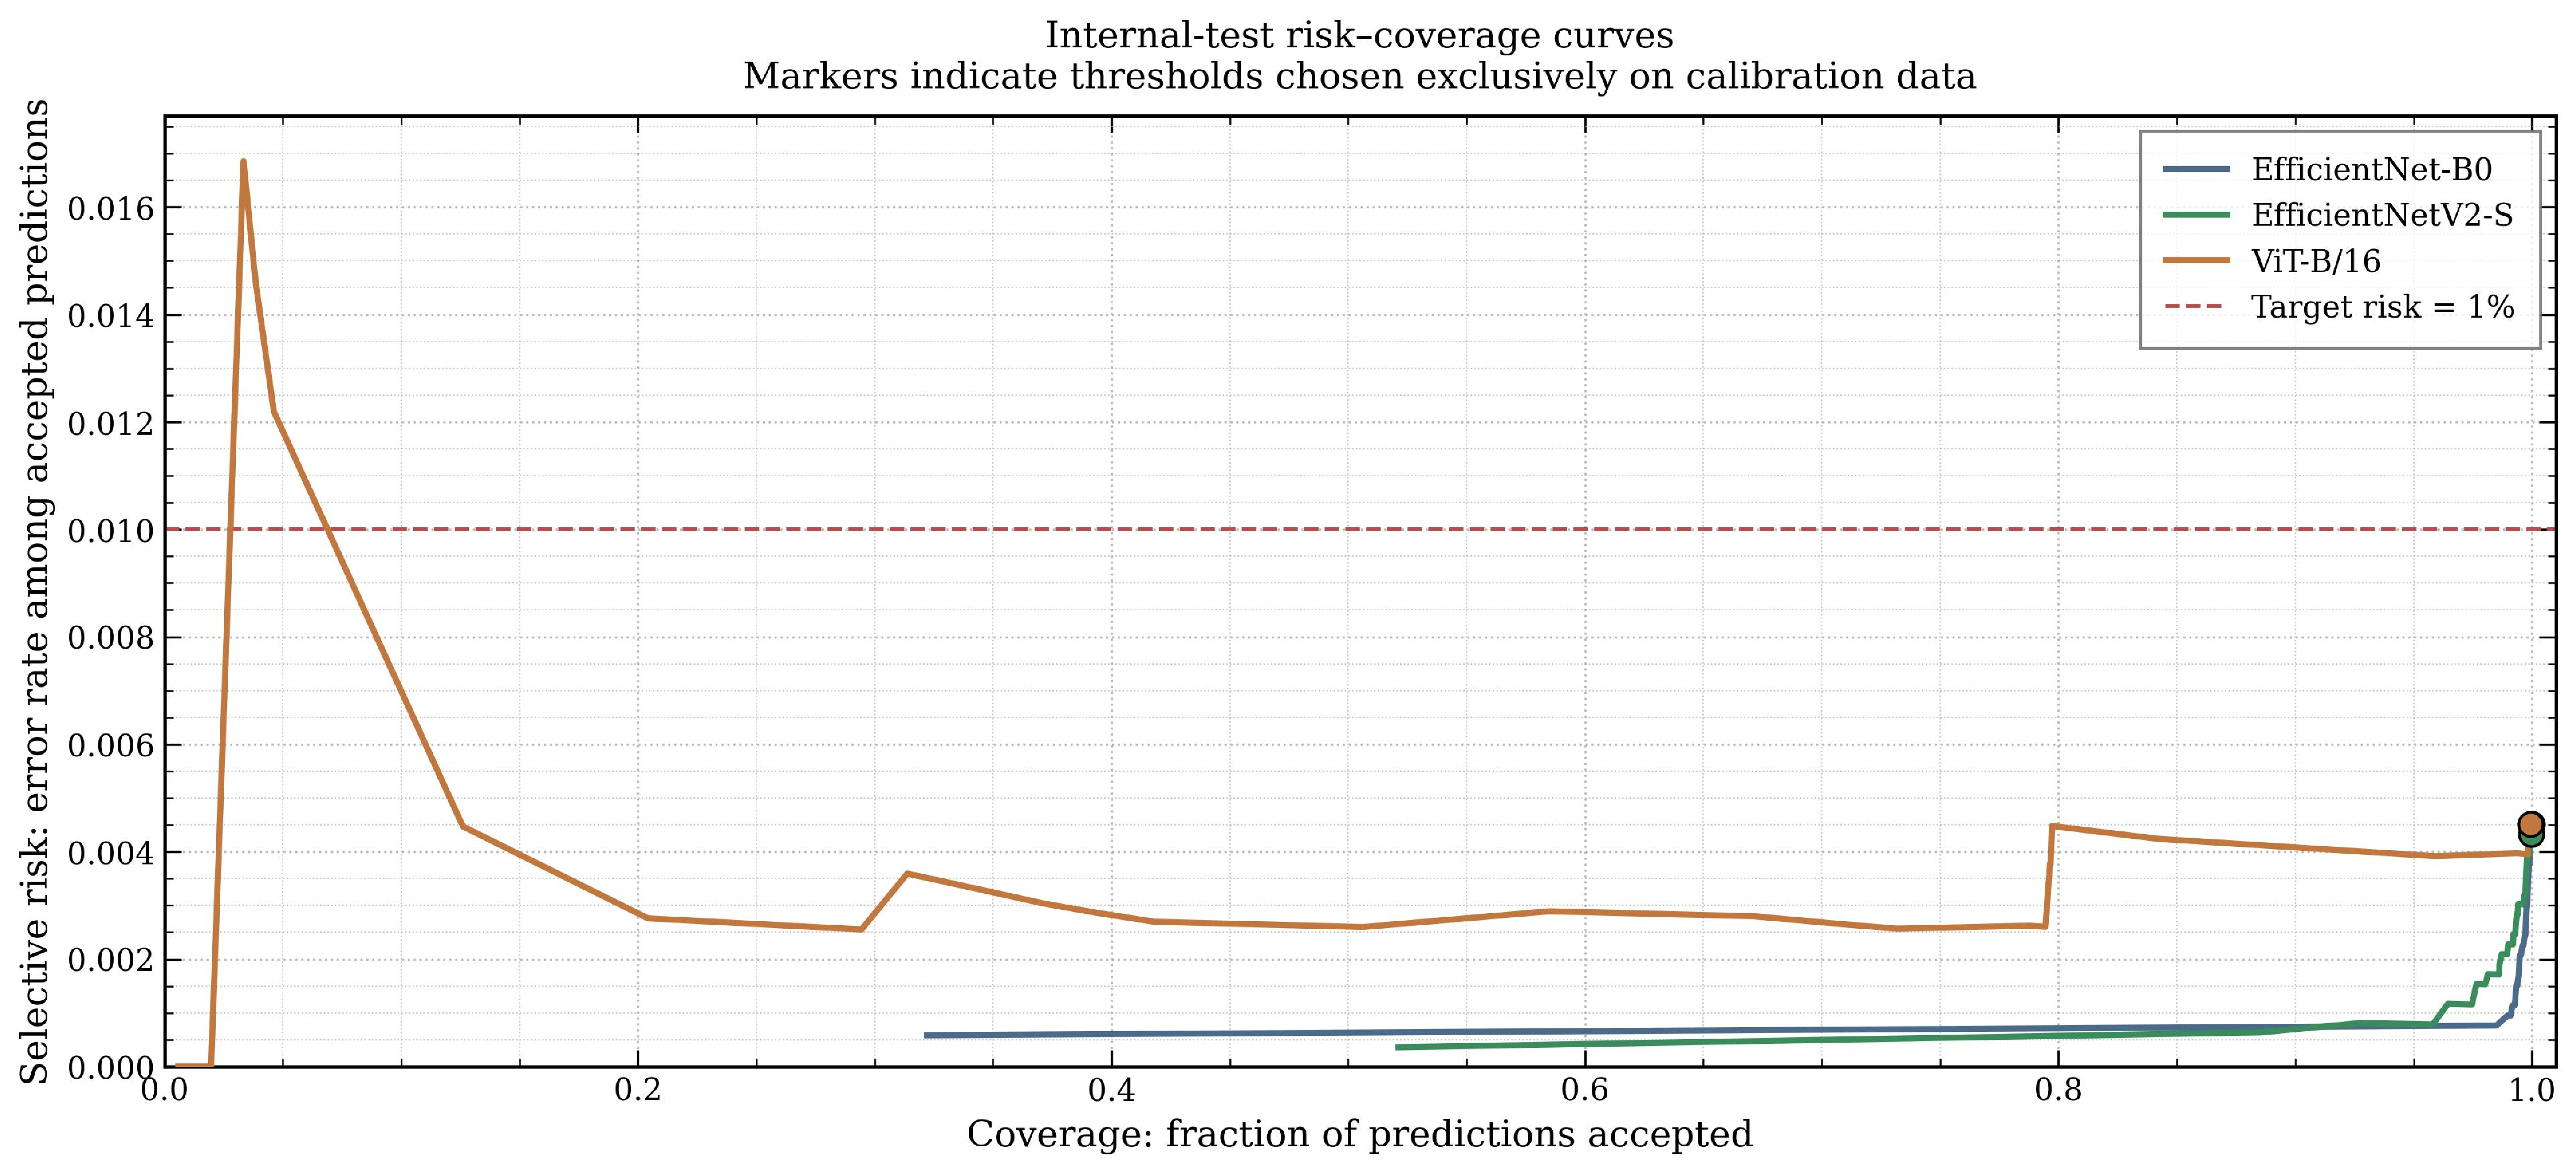
\includegraphics[
        width=0.94\textwidth,
        height=0.42\textheight,
        keepaspectratio
    ]{fig_05_risk_coverage_curves.pdf}
    \caption{Risk--coverage curves on the Main19 internal test set
    (5{,}322~images) for all three classifiers. Risk is the top-1
    error rate among accepted predictions. The vertical dashed line
    marks the confidence threshold ($\bm{\tau}\!=\!0.50$) selected
    using the calibration partition only. At this threshold,
    EfficientNet-B0 accepts all images (coverage~100\%). Confidence
    values are uncalibrated softmax outputs.}
    \label{fig:risk_coverage}
\end{figure*}

\begin{table*}[!t]
\caption{Selective-Prediction Results on the Main19 Internal Test Set
(5{,}322~images). The confidence threshold was selected on
calibration data only ($\bm{\tau}\!=\!0.50$, the minimum floor).
Coverage denotes the fraction of test images accepted; risk denotes
the top-1 error rate among accepted images. Confidence: uncalibrated
softmax.}
\label{tab:selective}
\centering
\small
\setlength{\tabcolsep}{8pt}
\renewcommand{\arraystretch}{1.12}
\begin{tabular}{lccccc}
\toprule
\textbf{Model} & \textbf{Threshold} & \textbf{Coverage} & \textbf{Rejected} & \textbf{Selective Acc.} & \textbf{Risk} \\
\midrule
EfficientNet-B0 & 0.50 & 1.0000 & 0 & 0.9955 & 0.0045 \\
EfficientNetV2-S & 0.50 & 0.9996 & 2 & 0.9957 & 0.0043 \\
ViT-B/16 & 0.50 & 0.9994 & 3 & 0.9955 & 0.0045 \\
\bottomrule
\end{tabular}
\end{table*}

\subsection{Heuristic Visible Lesion-Area Proxy}

The heuristic visible lesion-area proxy was computed for all Main19
images across training, calibration, and internal test splits (total:
20{,}562 images, excluding healthy classes for lesion interpretation
but including them in the computation pool).
Fig.~\ref{fig:lesion} presents a qualitative panel.

\begin{figure*}[!t]
    \centering
    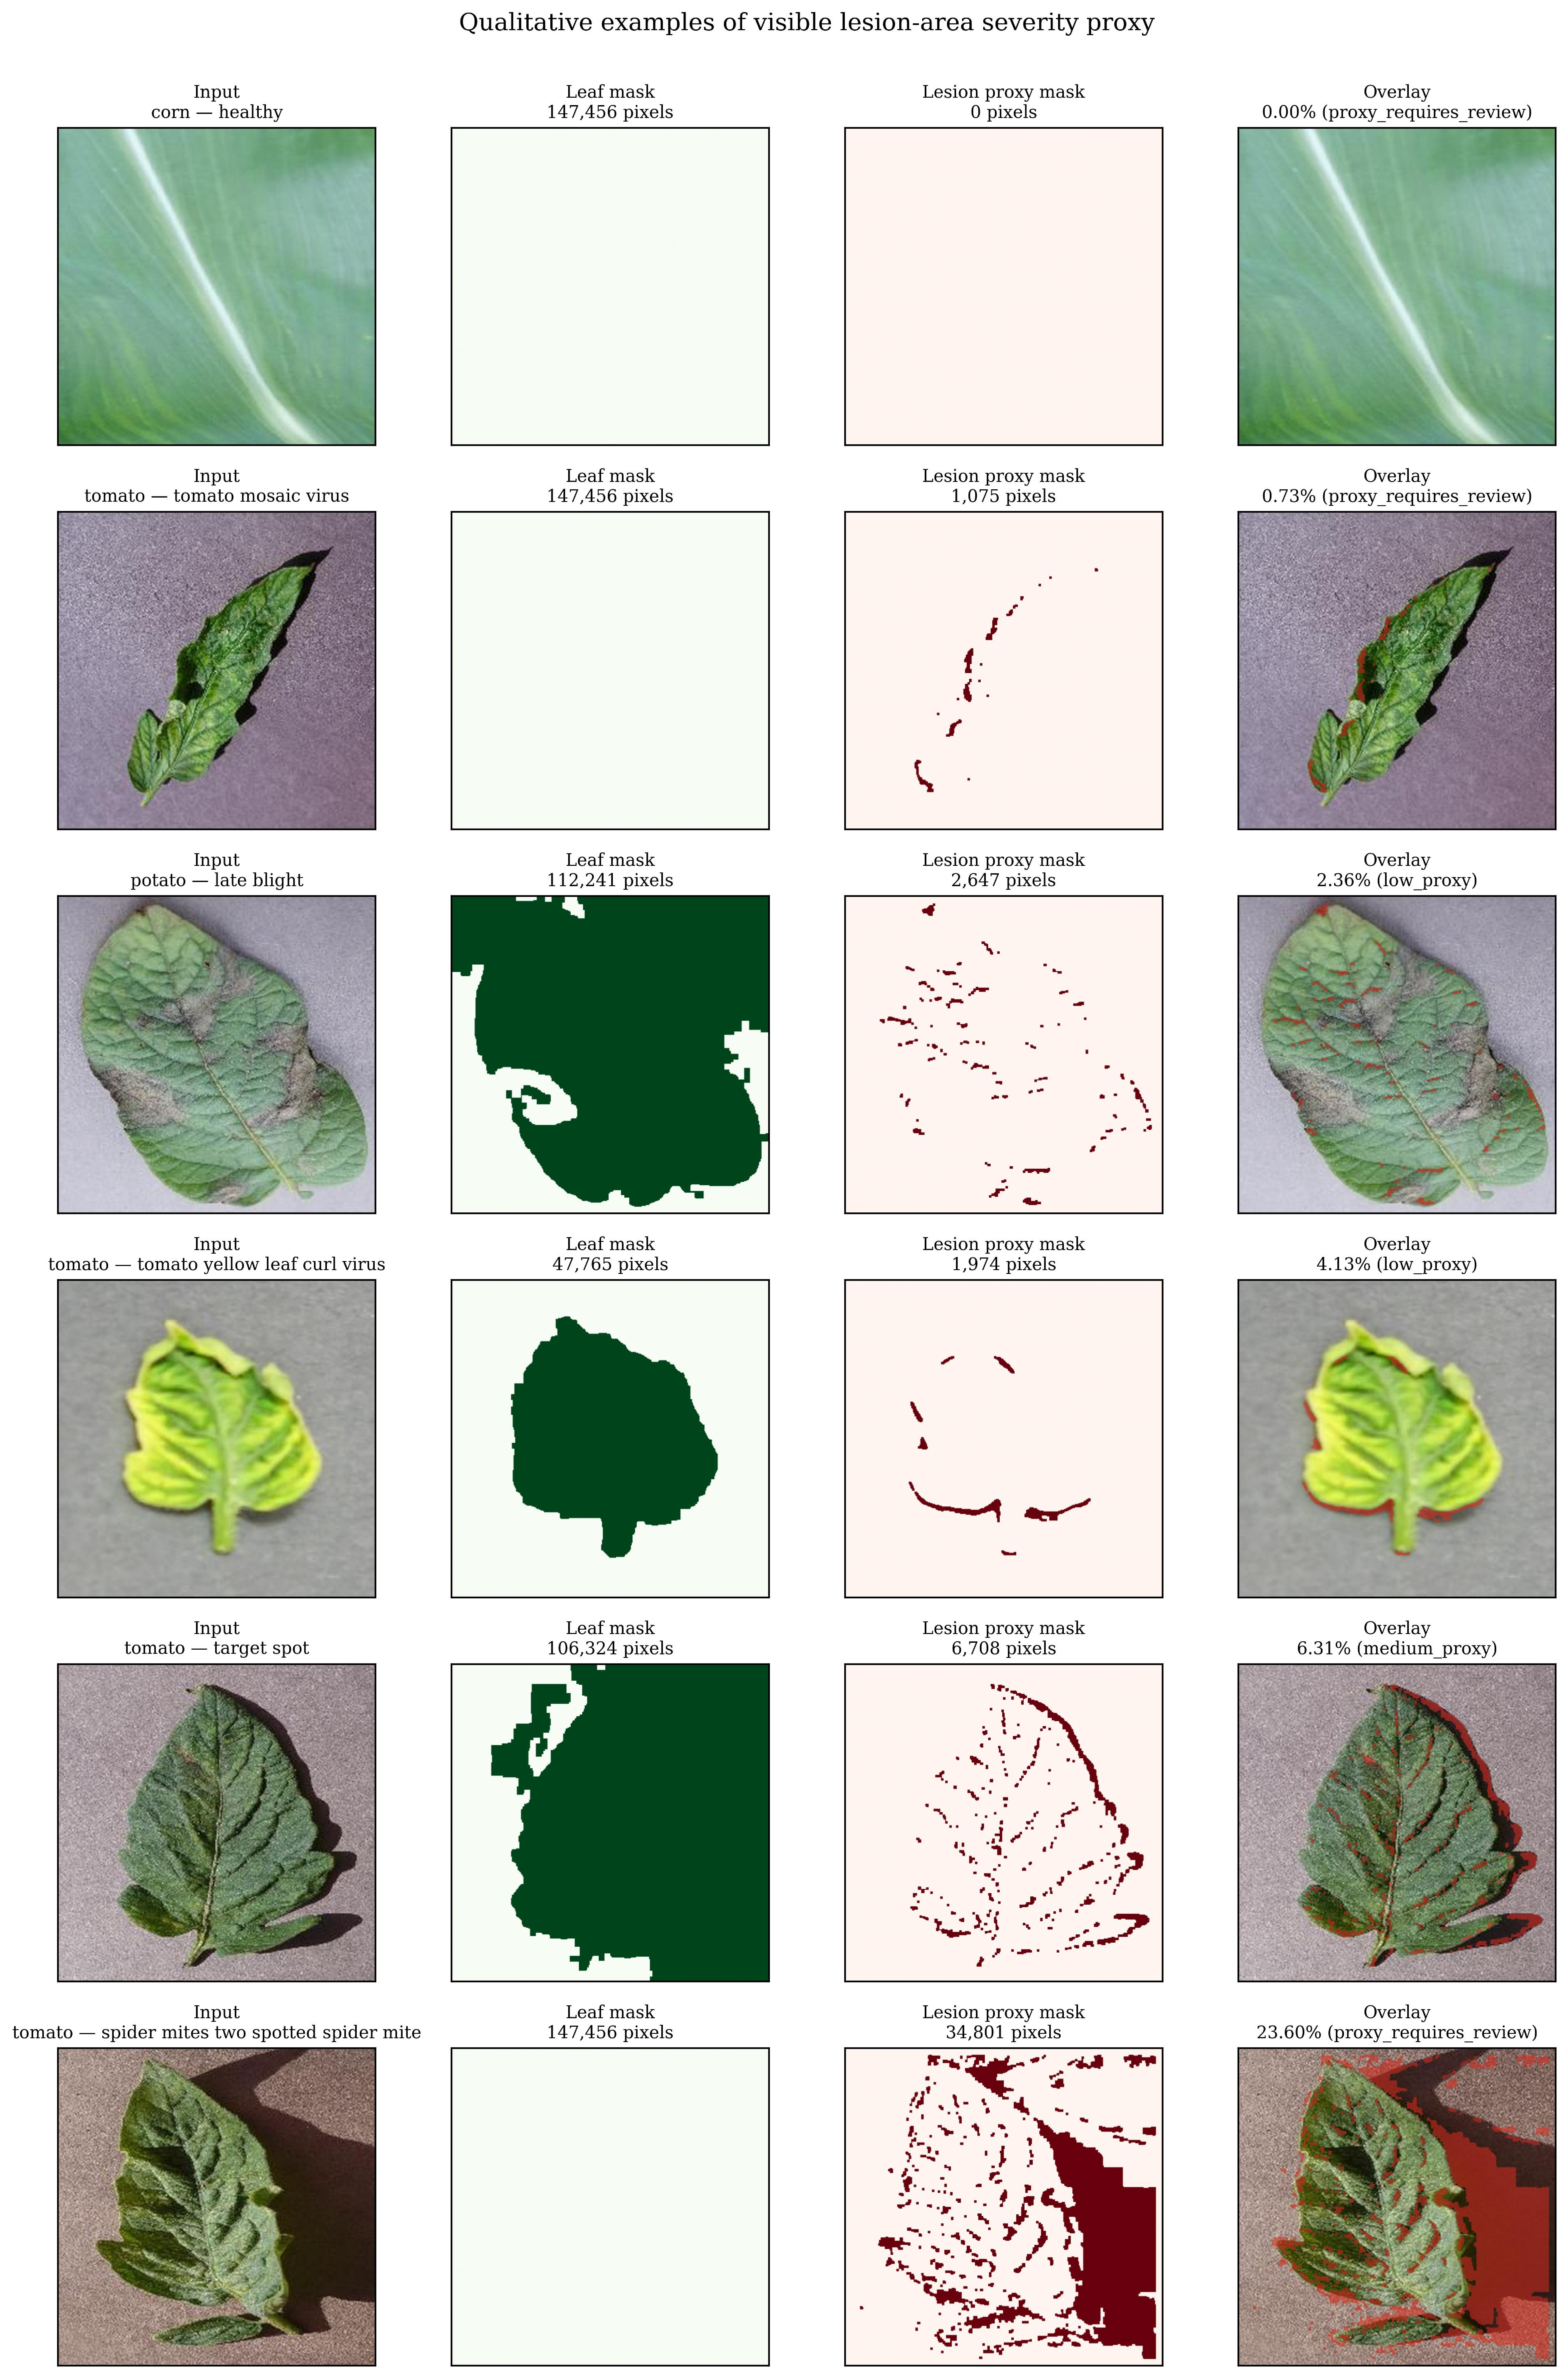
\includegraphics[
        width=0.94\textwidth,
        height=0.45\textheight,
        keepaspectratio
    ]{fig_06_lesion_severity_proxy.pdf}
    \caption{Qualitative examples of the heuristic image-based visible
    lesion-area proxy. Highlighted pixels satisfy pre-defined
    lesion-like colour/texture criteria. The mild ($<$5\%), moderate
    (5--20\%), and severe ($>$20\%) labels are proxy bands only; this
    procedure is not expert-annotated segmentation, a model attention
    map, or an agronomically validated disease-severity estimate.}
    \label{fig:lesion}
\end{figure*}

Across splits, mean visible lesion area is approximately 6.2\%
(calibration: 6.19\%; internal test: 6.22\%; training: 6.26\%), with
a median of approximately 4.4\% and standard deviation of
approximately 6.5\%. The close agreement across splits indicates that
partition stratification preserved lesion-area distributions.

Notable class-level variation is observed. Classes with large proxy
lesion areas include potato early blight (mean 12.47\%), corn gray
leaf spot (13.01\%), and corn northern leaf blight (11.42\%). Classes
with smaller proxy areas include tomato mosaic virus (1.79\%), corn
healthy (0.86\%), and tomato healthy (2.73\%). These differences are
qualitatively plausible given the known visual symptom morphology of
each condition---early blight and late blight produce large necrotic
lesions, whereas mosaic virus primarily causes colour mottling without
prominent discrete lesion areas. However, these observations do not
constitute validation against expert-annotated lesion ground truth
and must not be interpreted as agronomically validated severity
estimates.

\subsection{External Domain Shift on PlantDoc}
\label{sec:plantdoc}

The EfficientNet-B0 baseline was applied zero-shot to the 144-image,
15-class semantically mapped PlantDoc external test subset. The
results reveal severe domain shift.

\textbf{Overall metrics.}
Top-1 accuracy: \textbf{0.1944} (28 of 144 correct). Balanced
accuracy: 0.1998. Macro-F1: 0.1428. Weighted-F1: 0.1698. Top-5
accuracy: \textbf{0.6736}.

The contrast with internal performance (99.53\% top-1 accuracy) is
stark: the model was trained on controlled, single-leaf images against
uniform backgrounds, while PlantDoc contains field-acquired images
with complex natural backgrounds, variable lighting, and co-occurring
foliage.

\textbf{Top-5 analysis.}
The high top-5 accuracy (67.4\%) indicates that the correct class is
retrievable within the model's top-5 predictions for the majority of
images, even when it is not the top-ranked class. This suggests that
the model retains some ability to distinguish relevant disease features
under domain shift, but that ranking confusion prevents reliable
top-1 identification.

\textbf{Confidence analysis.}
Despite poor accuracy, the model remains overconfident: mean
confidence on all 144 PlantDoc images is 0.845, with median 0.942.
Correct predictions have mean confidence 0.883; incorrect predictions
have mean confidence 0.836. The small gap (0.047) indicates that
confidence alone is insufficient to identify domain-shifted
misclassifications. When the source-domain selective threshold
($\bm{\tau}\!=\!0.50$) is applied, only 11 of 144 images are rejected
(coverage:~92.4\%) and retained-case accuracy improves only marginally
to 19.5\%. The calibration-derived threshold provides minimal
protection against domain-shift errors, confirming that source-domain
confidence thresholds do not provide sufficient protection under
severe external shift.

Fig.~\ref{fig:plantdoc_confidence} shows the confidence distributions
for correct and incorrect predictions on PlantDoc.

\begin{figure}[!t]
    \centering
    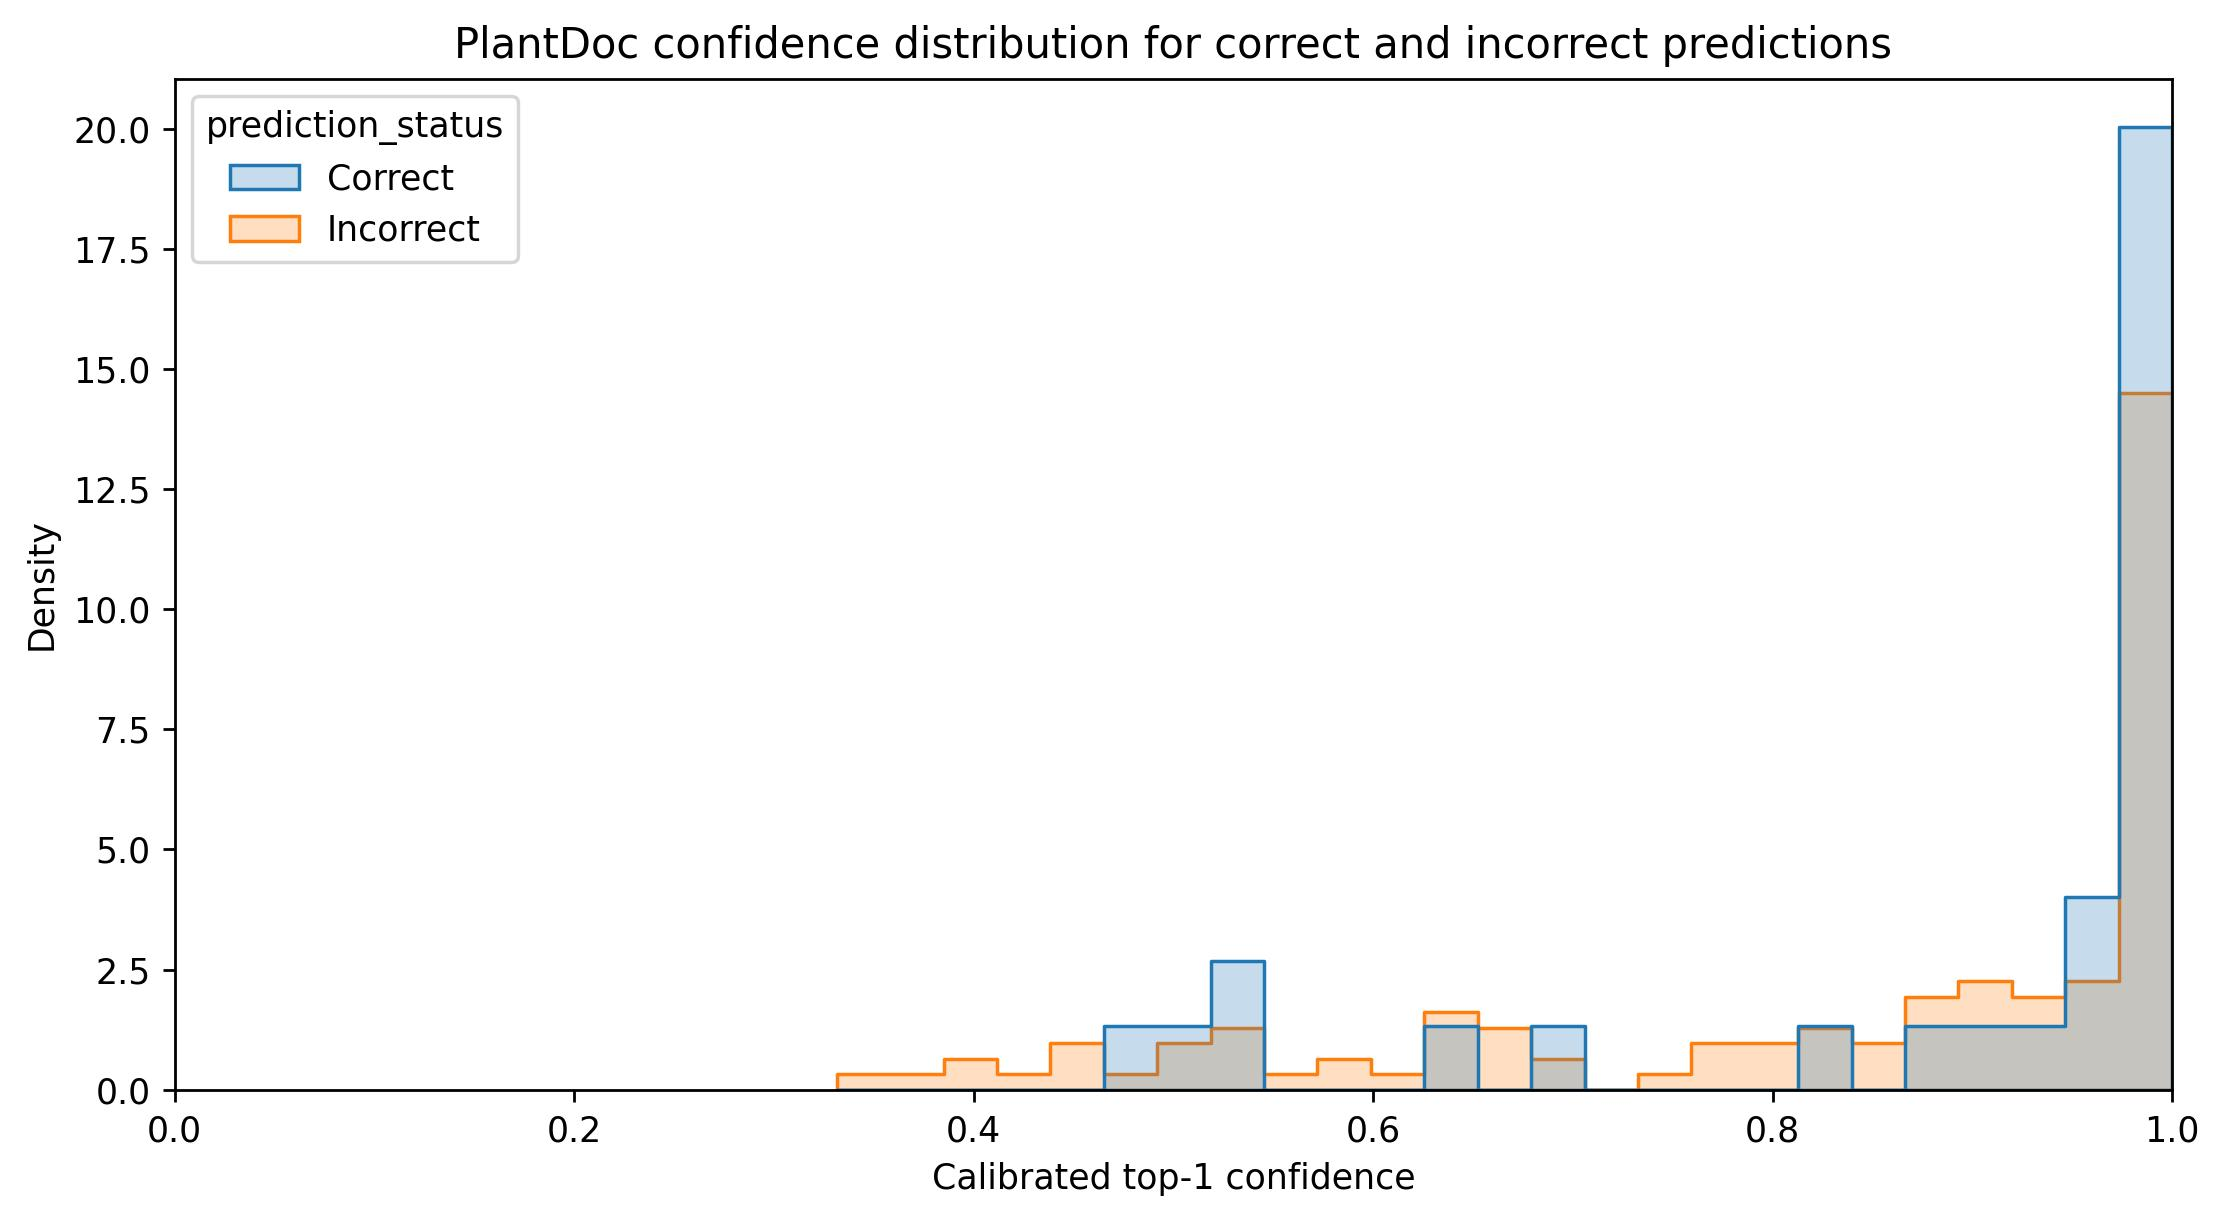
\includegraphics[
        width=\columnwidth,
        height=0.34\textheight,
        keepaspectratio
    ]{fig_09_plantdoc_confidence.pdf}
    \caption{Confidence distributions for correct (28) and incorrect
    (116) predictions on the PlantDoc external test set (144~images,
    EfficientNet-B0, $T\!=\!1.0$). The distributions overlap
    substantially, indicating that softmax confidence does not
    reliably distinguish correct from incorrect predictions under
    domain shift. Mean confidence: correct~0.883, incorrect~0.836.}
    \label{fig:plantdoc_confidence}
\end{figure}

Table~\ref{tab:plantdoc_overall} summarises the overall external
metrics.

\begin{table}[!t]
\caption{PlantDoc Zero-Shot External Evaluation Summary
(EfficientNet-B0, 144~images, 15~semantically mapped classes,
$T\!=\!1.0$).}
\label{tab:plantdoc_overall}
\centering
\small
\begin{tabular}{lr}
\toprule
\textbf{Metric} & \textbf{Value} \\
\midrule
Top-1 accuracy & 0.1944 \\
Top-5 accuracy & 0.6736 \\
Balanced accuracy & 0.1998 \\
Macro-F1 & 0.1428 \\
Weighted-F1 & 0.1698 \\
Mean confidence (all) & 0.845 \\
Median confidence (all) & 0.942 \\
Mean confidence (correct) & 0.883 \\
Mean confidence (incorrect) & 0.836 \\
\bottomrule
\end{tabular}
\end{table}

\textbf{Per-class and per-crop analysis.}
Table~\ref{tab:plantdoc_perclass} presents the per-class PlantDoc
results. Six of 15 classes achieve zero correct top-1 predictions.
At the crop level, bell~pepper achieves the highest top-1 accuracy
(0.353), followed by corn (0.269), potato (0.182), and tomato (0.139).
Fig.~\ref{fig:plantdoc_confusion} shows the external-domain confusion
matrix. Fig.~\ref{fig:plantdoc_crop} shows top-1 accuracy by crop.

\begin{table*}[!t]
\caption{PlantDoc-to-Main19 Semantic Class Mapping and Per-Class
Zero-Shot Results. $^\dagger$Folder-to-healthy mappings are semantic
assumptions. Six classes achieve zero top-1 accuracy. Twelve PlantDoc
folders covering crops absent from Main19 were excluded.}
\label{tab:plantdoc_perclass}
\centering
\small
\setlength{\tabcolsep}{5pt}
\renewcommand{\arraystretch}{1.12}
\begin{tabular}{llrrr}
\toprule
\textbf{PlantDoc Folder} & \textbf{Mapped Main19 Label} & \textbf{Imgs} & \textbf{Top-1} & \textbf{F1} \\
\midrule
Bell\_pepper\_leaf$^\dagger$ & bell\_pepper\_\_healthy & 8 & 0.750 & 0.240 \\
Bell\_pepper\_leaf\_spot & bell\_pepper\_\_bacterial\_spot & 9 & 0.000 & 0.000 \\
Corn\_Gray\_leaf\_spot & corn\_\_cercospora\_leaf\_spot & 4 & 0.500 & 0.250 \\
Corn\_rust\_leaf & corn\_\_common\_rust & 10 & 0.200 & 0.235 \\
Corn\_leaf\_blight & corn\_\_northern\_leaf\_blight & 12 & 0.250 & 0.333 \\
Potato\_leaf\_early\_blight & potato\_\_early\_blight & 14 & 0.286 & 0.381 \\
Potato\_leaf\_late\_blight & potato\_\_late\_blight & 8 & 0.000 & 0.000 \\
Tomato\_leaf$^\dagger$ & tomato\_\_healthy & 8 & 0.000 & 0.000 \\
Tomato\_leaf\_bacterial\_spot & tomato\_\_bacterial\_spot & 9 & 0.000 & 0.000 \\
Tomato\_Early\_blight\_leaf & tomato\_\_early\_blight & 9 & 0.111 & 0.133 \\
Tomato\_leaf\_late\_blight & tomato\_\_late\_blight & 10 & 0.600 & 0.279 \\
Tomato\_mold\_leaf & tomato\_\_leaf\_mold & 6 & 0.000 & 0.000 \\
Tomato\_Septoria\_leaf\_spot & tomato\_\_septoria\_leaf\_spot & 12 & 0.167 & 0.211 \\
Tomato\_leaf\_mosaic\_virus & tomato\_\_tomato\_mosaic\_virus & 10 & 0.000 & 0.000 \\
Tomato\_leaf\_yellow\_virus & tomato\_\_yellow\_leaf\_curl\_virus & 15 & 0.133 & 0.222 \\
\midrule
\multicolumn{2}{l}{\textbf{Total (15 compatible classes)}} & \textbf{144} & \textbf{0.194} & \textbf{0.143} \\
\bottomrule
\end{tabular}
\end{table*}

\begin{figure}[!t]
    \centering
    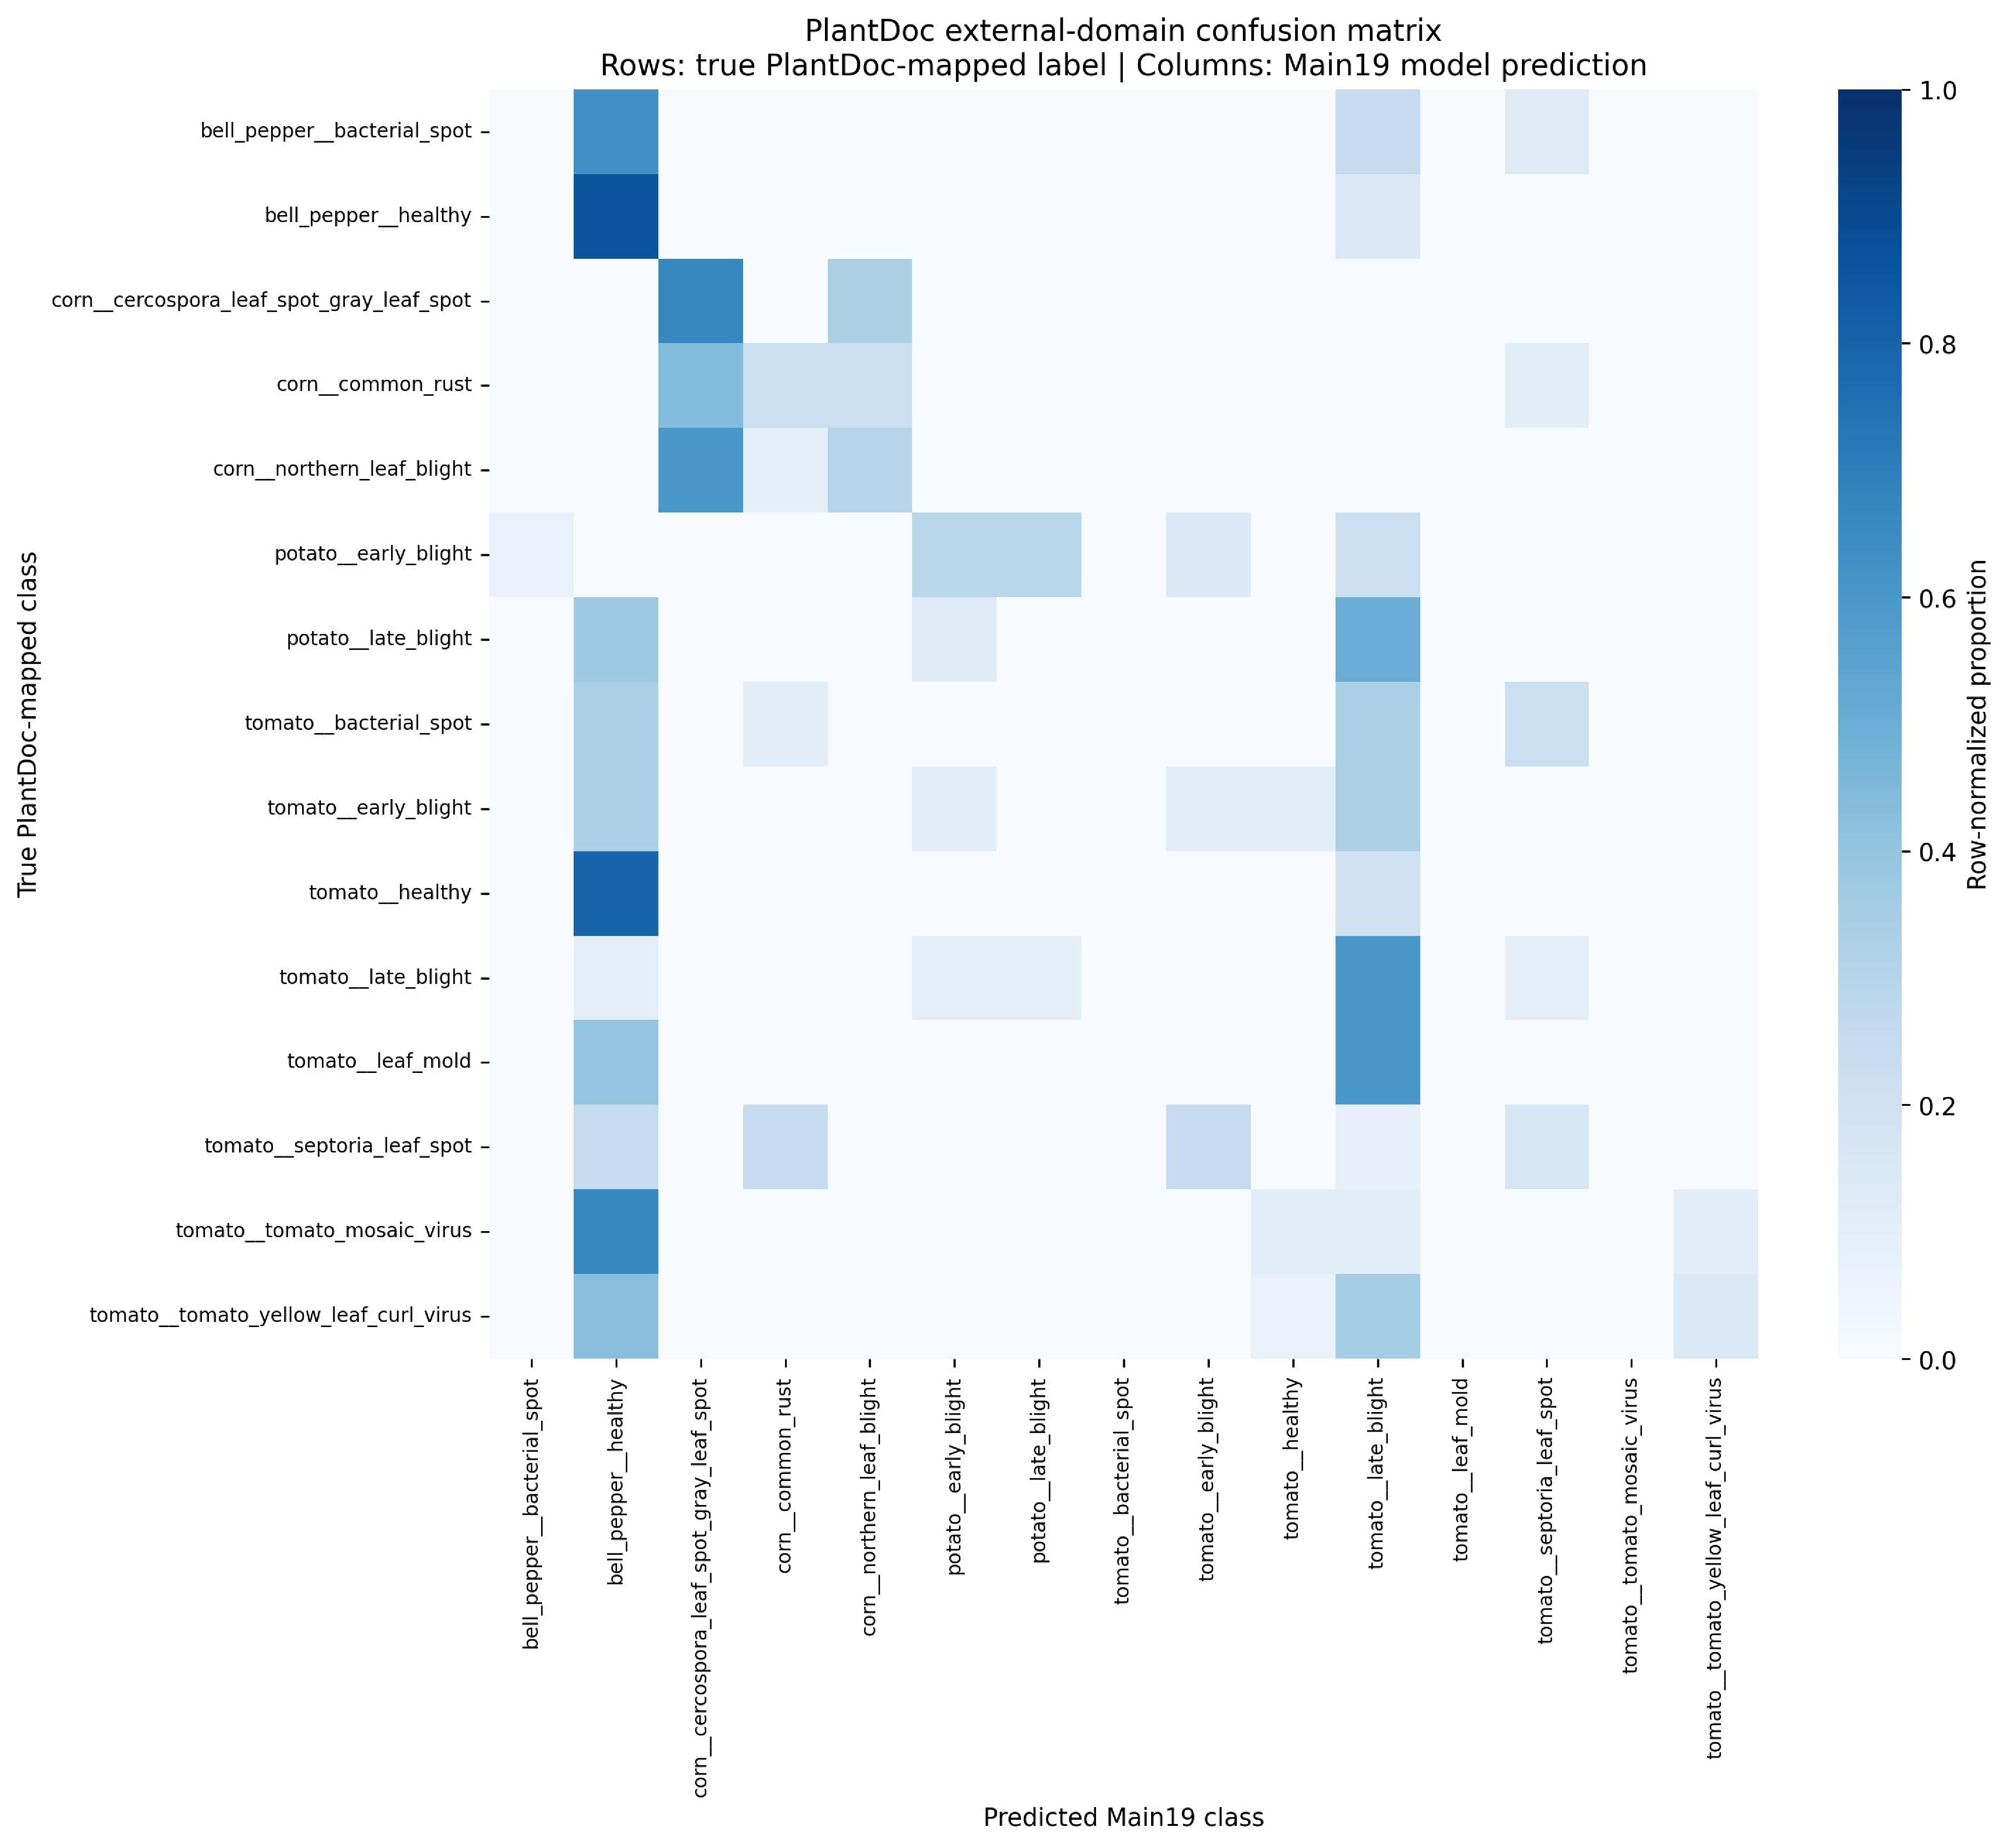
\includegraphics[
        width=\columnwidth,
        height=0.47\textheight,
        keepaspectratio
    ]{fig_07_plantdoc_confusion_matrix.pdf}
    \caption{Confusion matrix for EfficientNet-B0 on the semantically
    mapped PlantDoc external test subset (144~images). Rows: 15
    PlantDoc-mapped true labels. Columns: Main19 predicted labels.
    The model outputs predictions across all 19~Main19 classes;
    6~classes never appear as predictions on this subset. The low
    diagonal density confirms severe top-1 accuracy degradation under
    domain shift.}
    \label{fig:plantdoc_confusion}
\end{figure}

\begin{figure}[!t]
    \centering
    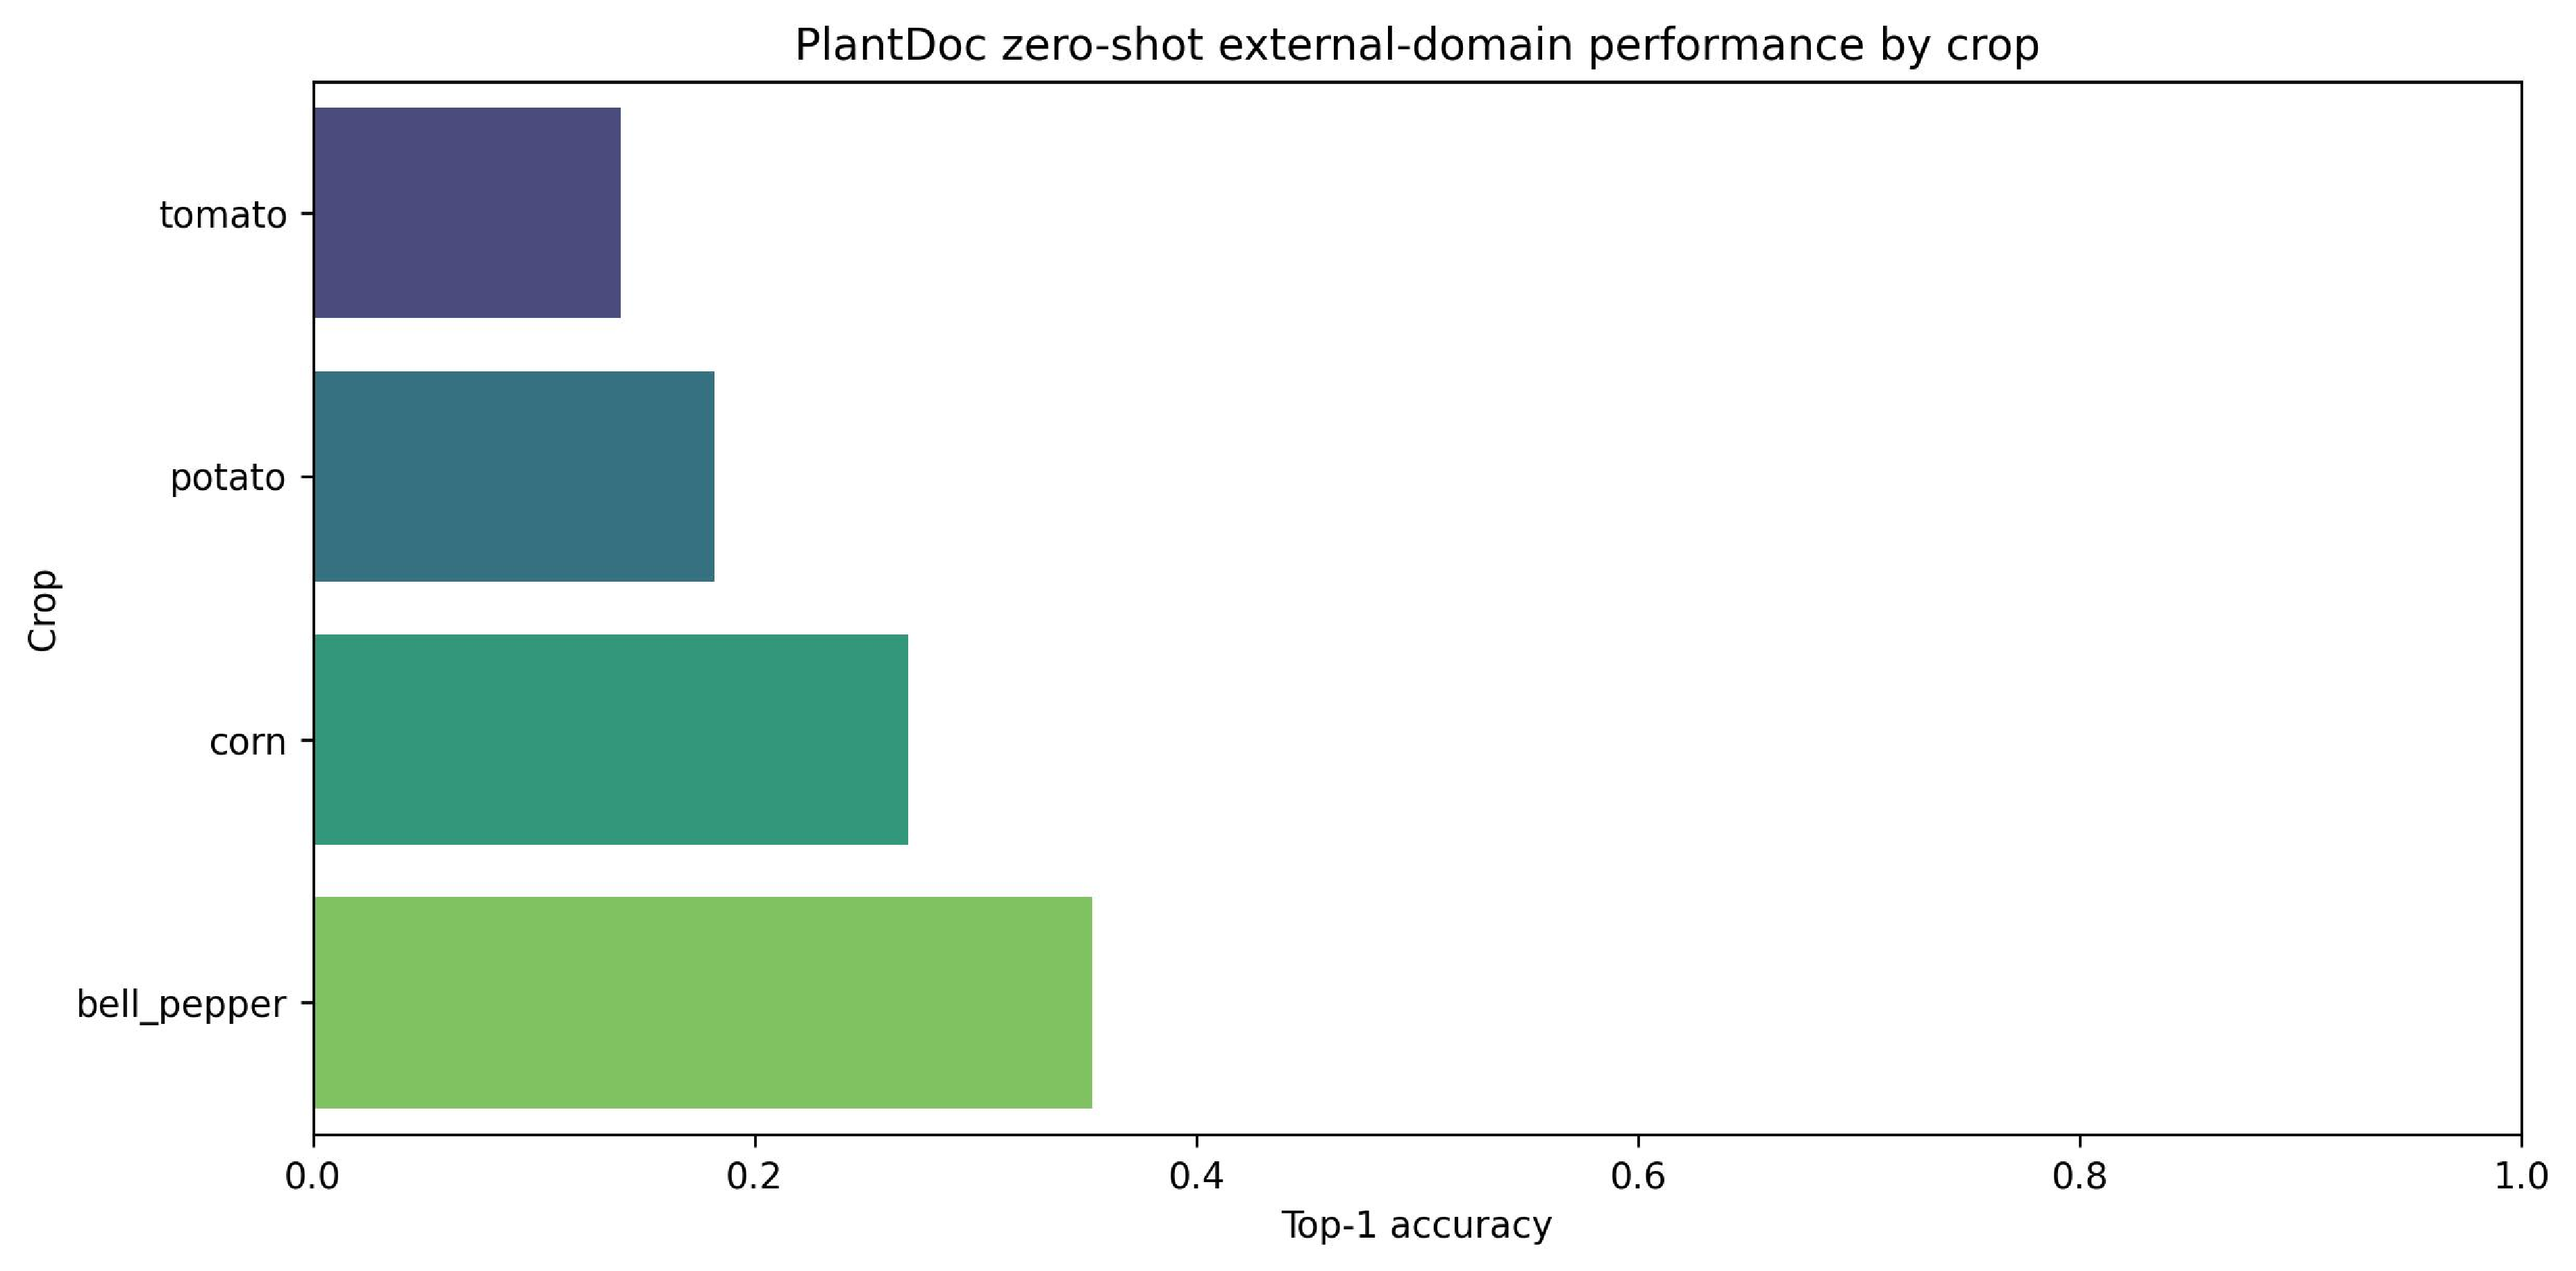
\includegraphics[
        width=\columnwidth,
        height=0.30\textheight,
        keepaspectratio
    ]{fig_10_plantdoc_accuracy_by_crop.pdf}
    \caption{PlantDoc zero-shot top-1 accuracy grouped by crop in the
    semantically mapped external subset. Crop-level values should be
    interpreted cautiously because crop groups differ in image count
    and number of mapped classes.}
    \label{fig:plantdoc_crop}
\end{figure}

The PlantDoc result should be interpreted as evidence of substantial
source-to-target domain shift within the evaluated mapped subset,
rather than as a direct estimate of universal field-deployment
performance across crops, regions, cultivars, devices, and agronomic
conditions.

\subsection{Retrieval-Grounded Advisory Prototype Evaluation}

The prototype was functionally tested for deterministic recovery of
the label-associated advisory entry and for enforcement of
confidence-policy rules across all 19 supported labels in English,
Hindi, and Telugu. All 19~labels retrieved the correct primary
advisory entry (19/19 deterministic primary-entry recovery in a
closed-label functional test). Advisory responses ranged from
1{,}568 to 1{,}914~characters at the medium-confidence tier,
covering symptom descriptions, causal agents, and management
principles.

These tests verify system routing and policy behaviour; they do not
constitute expert validation of agronomic advice, farmer
comprehension, translation quality, or user-facing evaluation.
Table~\ref{tab:rag_validation} summarises the functional test
results.

\begin{table}[!t]
\caption{Retrieval-Grounded Advisory Prototype: Functional Test
Summary. The 19/19 label-match result reflects deterministic routing
in a closed-label test, not open-query retrieval performance.}
\label{tab:rag_validation}
\centering
\small
\begin{tabular}{ll}
\toprule
\textbf{Property} & \textbf{Value} \\
\midrule
Knowledge base entries & 19 \\
Primary label recovery & 19/19 (deterministic) \\
Languages & English, Hindi, Telugu \\
Advisory length range & 1{,}568--1{,}914 chars \\
Retrieval method & TF-IDF cosine similarity \\
Pesticide prescription & Prohibited \\
Expert confirmation ($<$0.70) & Required \\
Field-verification ($\geq$0.90) & Mandatory warning \\
KB entries expert-reviewed & No \\
\bottomrule
\end{tabular}
\end{table}

% =====================================================================
\section{Discussion}
\label{sec:discussion}
% =====================================================================

\subsection{Controlled-Domain Performance in Context}

The EfficientNet-B0 baseline achieves 99.53\% top-1 accuracy on the
locked internal test set---a result consistent with the broader
literature on PlantVillage
models~\cite{mohanty2016deep,too2019comparative,ferentinos2018deep}.
However, this study deliberately places this result in context: it is
a ceiling observed under matched imaging conditions, not a guarantee
of field-level performance.

Under the evaluated models and split protocol, larger architectures
did not show a practically meaningful internal-domain advantage over
EfficientNet-B0. All three models achieved accuracy above 99.3\% and
macro-F1 above 0.992, with parameter counts ranging from
${\approx}5.3$\,M (B0) to 85.8\,M (ViT-B/16). The near-identical
performance suggests that the discriminative features required for
near-perfect classification on this controlled task are accessible to
all three architectures, and the differentiating factors become
calibration quality, parameter efficiency, and generalisation under
shift.

\subsection{Calibration: Metric-Dependent Improvement}

Temperature scaling with $T\!=\!1.5695$ reduced internal-test ECE
by~29\% (from 0.00321 to 0.00228) and Brier score from 0.00704 to
0.00642, but NLL increased slightly from 0.01550 to 0.01593.
This mixed result underscores that calibration quality depends on the
specific metric used to assess it. The ECE and Brier improvements are
consistent with the model's confidence distribution being softened
toward the identity diagonal on the reliability curve. The slight NLL
increase may reflect the trade-off between bin-level calibration and
pointwise log-likelihood.

The PlantDoc confidence analysis reveals a critical limitation of
calibration under distribution shift: despite being calibrated on
PlantVillage data, the model assigns high confidence (median 0.942)
to most PlantDoc images, including a large majority of misclassified
ones. The mean confidence gap between correct and incorrect external
predictions (0.047) is negligible. This finding confirms that
post-hoc calibration on source-domain data does not generalise to
target-domain confidence
estimates~\cite{ovadia2019can,guo2017calibration}.

\subsection{The External Domain Shift Gap}

The 80.1~percentage-point drop in top-1 accuracy between the internal
test (99.53\%) and the PlantDoc external test (19.44\%) is the most
important finding of this study. The PlantDoc subset comprises only
144~images from 15~classes (mean 9.6~per class), and several classes
contain as few as 4~images. Conclusions about specific class
difficulty must therefore be made cautiously.

Nevertheless, the result is consistent with published external
evaluations of PlantVillage-trained models on
PlantDoc~\cite{singh2020plantdoc} and reinforces
that the controlled-domain accuracy advantage does not transfer
reliably. The top-5 accuracy of 67.4\% suggests that the model has
not lost all discriminative knowledge: the correct answer is within
the model's top five candidates for most images. This provides a
basis for designing human-in-the-loop systems that present multiple
candidate diagnoses rather than forcing a single output.

When transferred to PlantDoc, the source-domain threshold
($\bm{\tau}\!=\!0.50$) rejected only 11 of 144 images and improved
retained-case accuracy only marginally, indicating that source-domain
confidence thresholds did not provide sufficient protection under
severe external shift.

\subsection{Lesion Proxy Limitations}

The heuristic visible lesion-area proxy provides a lightweight
image-characterisation mechanism that does not require a separate
segmentation model. The class-level patterns are qualitatively
plausible given known visual symptom morphology. However, the proxy
has not been validated against expert-annotated lesion masks, and its
heuristic colour/texture rules may confound image artefacts, natural
leaf variation, or reflection with pathological tissue. The proxy
should be treated as an exploratory tool for qualitative analysis and
future annotation prioritisation, not as a disease severity estimator.
It does not identify causal model features and does not constitute
classifier-attention analysis.

\subsection{Advisory Prototype and Responsible Deployment}

The retrieval-grounded advisory prototype addresses the gap between
classification output and usable field guidance. By conditioning
advisory content on classifier confidence and explicitly enforcing a
no-pesticide-prescription policy, the system avoids the most dangerous
overclaims possible from an automated diagnosis system. The
three-language support (English, Hindi, Telugu) begins to address the
multilingual needs of the primary intended user base.

However, the knowledge base was authored for this project and has not
been reviewed or endorsed by professional plant pathologists. TF-IDF
retrieval is sensitive to vocabulary and lacks semantic understanding.
The 19/19 primary-entry recovery result reflects deterministic
routing in a closed-label test, not competitive retrieval over a
large corpus. A rigorous evaluation would require expert review of
advisory quality, field user studies, translation quality assessment,
and adversarial testing with out-of-domain inputs.

\subsection{Limitations}

\textit{Controlled source data.}
PlantVillage images were collected under laboratory conditions. The
demonstrated external performance (19.44\% top-1 on PlantDoc)
confirms that this fundamentally limits generalisation.

\textit{Non-exhaustive near-duplicate audit.}
Of 136 pHash near-duplicate candidates, only 2 were reviewed and
confirmed as leakage; 134 remain unreviewed. The final partitions
are therefore not guaranteed to be completely free of near-duplicate
cross-split contamination.

\textit{PlantDoc mapping assumptions.}
Mapping PlantDoc folder names to Main19 classes required semantic
interpretation. The mappings of \texttt{Tomato\_leaf} to
\texttt{tomato\_\_healthy} and \texttt{Bell\_pepper\_leaf} to
\texttt{bell\_pepper\_\_healthy} are assumptions. Mapping errors
would affect class-level metrics.

\textit{PlantDoc subset size.}
With only 144 images across 15 classes (mean 9.6 per class),
class-level PlantDoc metrics have high variance and should be
interpreted with caution.

\textit{Cross-notebook metric discrepancy.}
EfficientNet-B0 internal-test accuracy differs by one prediction
between Notebook~04 (0.9953) and Notebook~07 (0.9955), and the
Brier scores differ by a factor of~20, indicating different
computation implementations. Cross-model Brier comparisons are
therefore not reported.

\textit{Missing V2-S temperature-scaled test metrics.}
Temperature-scaled internal-test evaluation was conducted only for
EfficientNet-B0. No temperature-scaled cross-model comparison is
possible.

\textit{Proxy validation.}
The visible lesion-area proxy has not been validated against
expert-annotated ground truth. All proxy band assignments are
heuristic.

\textit{Advisory evaluation depth.}
The advisory prototype was tested only for structural correctness
(label routing and policy enforcement). Agronomic quality, user
comprehension, translation accuracy, and safety under adversarial
inputs have not been evaluated.

\textit{No statistical significance tests.}
No confidence intervals or significance tests were computed.
Differences between closely performing models should not be
interpreted as statistically meaningful.

% =====================================================================
\section{Conclusion}
\label{sec:conclusion}
% =====================================================================

This paper presents a reproducible, leakage-aware crop disease
classification pipeline evaluated across controlled and external
domains. The principal finding is that high controlled-domain
accuracy---here 99.53\% for EfficientNet-B0 on Main19---does not
transfer to field-like imagery: zero-shot evaluation on a
semantically mapped PlantDoc subset yields 19.44\% top-1 accuracy
despite a top-5 accuracy of 67.4\%. Strong controlled-domain
performance did not transfer reliably to the semantically mapped
PlantDoc external subset, demonstrating that high internal accuracy
alone is insufficient evidence of robustness to field-like imaging
conditions.

Post-hoc temperature scaling ($T\!=\!1.5695$) reduced ECE from
0.00321 to 0.00228 and Brier score from 0.00704 to 0.00642 on the
internal test set, while NLL increased slightly from 0.01550 to
0.01593; calibration improvement was metric-dependent. Selective
prediction with a calibration-derived threshold of 0.50 achieved
full coverage at sub-0.5\% risk internally, but provided only
marginal protection against domain-shift errors externally. The
heuristic visible lesion-area proxy revealed qualitatively plausible
class-level variation in visible lesion area, while its limitations
as an unvalidated heuristic are explicitly documented.

The retrieval-grounded multilingual advisory prototype was
functionally tested for deterministic label-associated entry recovery
and confidence-policy enforcement. It was not evaluated for expert
agronomic correctness, farmer comprehension, or safety under
adversarial and out-of-domain inputs.

Future directions include: domain adaptation pre-training on
unlabelled field imagery; collection of expert-validated lesion
annotations to upgrade the lesion proxy; expansion of the PlantDoc
evaluation to more crops and regions; completion of the near-duplicate
audit for remaining unreviewed candidates; and rigorous field user
studies of the advisory system with professional agronomists.

% =====================================================================
\section*{Declarations}
% =====================================================================

\textit{Data availability.}
The PlantVillage dataset is publicly available at
\url{https://plantvillage.psu.edu/}. PlantDoc is available at
\url{https://github.com/pratikkayal/PlantDoc-Dataset}. The derived
split manifests, class maps, and evaluation metadata are available in
the project repository.

\textit{Code availability.}
All analysis notebooks and reproducibility artefacts are available in
the project repository at random seed~7 with
Python~3.12.13~/~PyTorch~2.10.0~/~torchvision~0.25.0.

\textit{Conflicts of interest.}
The authors declare no conflicts of interest.

\textit{Responsible-use statement.}
The advisory prototype described in this paper is designed for
educational and screening purposes only. It does not constitute a
confirmed agronomic or clinical diagnosis and must not be used to
prescribe pesticides, chemicals, or treatments without professional
agronomic review.

\textit{Acknowledgements.}
The authors acknowledge the use of Kaggle GPU resources for all model
training experiments.

\balance

\bibliographystyle{IEEEtran}
\bibliography{references}

\end{document}
